\documentclass[a4paper]{article}

\usepackage{listings}
\usepackage[utf8]{inputenc}
\usepackage[T1]{fontenc}
\usepackage[spanish]{babel}
\usepackage[left=2cm, right=2cm, top=2cm, bottom=2cm]{geometry}
\usepackage{setspace}
\usepackage{graphicx}
\usepackage{xcolor}
\usepackage{geometry}
\usepackage{multirow}
\usepackage[hidelinks]{hyperref}
\usepackage{setspace} % Para el espaciado entre lineas
\setstretch{1.2} % Aquí definimos el espaciado en unidades
\usepackage{parskip} %  Para arreglar la forma en la que se manejan los parrafos
\usepackage{fancyhdr}
\usepackage{tikz,lipsum,lmodern}
\usepackage[most]{tcolorbox}
\usetikzlibrary{shapes.geometric, arrows}
\usepackage{appendix}
\usepackage{tocloft} % Paquete para personalizar el índice de figuras
%\usepackage{minted} % Paquete para resaltado de sintaxis

% Sets de dimensiones
\setlength{\parindent}{0pt}
\setlength{\parskip}{0.8em plus 0.5em minus 0.2em}
\setlength{\parfillskip}{\parindent plus 1fill}

% Declaración de variables personalizadas
\newcommand{\logoPortada}{Images/PixelartPisa.png}
\newcommand{\cifplogo}{Images/cifplogo.png}

% Definición de colores
\definecolor{bluePortada}{HTML}{146c8a}

%Adicionales
\setlength{\headheight}{40.2pt}
\pagestyle{fancy}
\fancyhf{}
\lhead{\includegraphics[width=1cm]{\logoPortada}}\rhead{
\includegraphics[width=2cm]{Images/cifplogo.png}}
\renewcommand{\headrulewidth}{3pt}
\renewcommand{\headrule}{\hbox to\headwidth{\color{bluePortada}\leaders\hrule height \headrulewidth\hfill}}

\tikzstyle{startstop}=[rectangle,rounded corners, minimum width=3cm,minimum height= 1cm, text centered,draw=black, fill=red]
\tikzstyle{io}=[trapezium,trapezium left angle=70,trapezium right angle=110,minimum width=3cm,minimum height= 1cm, text centered,draw=black, fill=blue]
\tikzstyle{process}=[rectangle,minimum width=3cm,minimum height= 1cm, text centered,text width= 3cm,draw=black, fill=orange]
\tikzstyle{decision}=[diamond,minimum width=3cm,minimum height= 1cm, text centered,draw=black, fill=green]
\tikzstyle{arrow}=[thick]



\begin{document} % Inicio del documento
\begin{titlepage}
    \centering % para centrar
    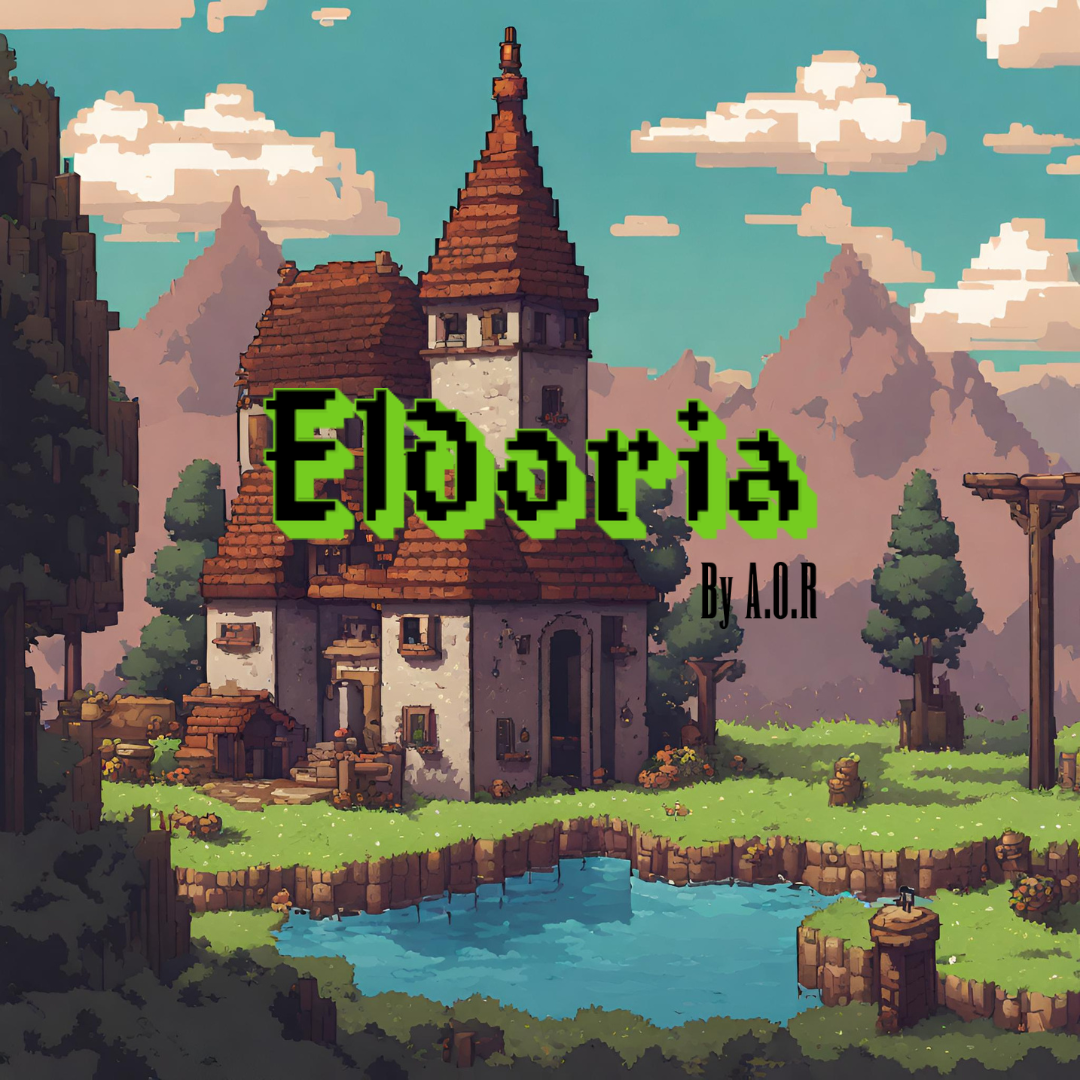
\includegraphics[width=0.5\textwidth]{Images/Eldoria.png}\par
    \vspace{0.4cm}
    {\scshape\LARGE\textbf{TFG DAM - CIFP LaLaboral}\par} % Contenido de la portada
    \vspace{0.4cm}
    {\LARGE\textcolor{bluePortada}{Eldoria - Alejandro Orviz Recalde}\par}
\end{titlepage}
% Comienzo del TOC
\clearpage

\tableofcontents
\clearpage

\listoffigures
\clearpage

\listoftables
\clearpage
% ---------------------------------------------------------------------
\section{Agradecimientos}
Este proyecto no sería posible sin la ayuda de varias personas involucradas en este desarrollo. Carles por ayudarme con sus reviews de código,
Laura por darme parte de sus conocimientos en el desarrollo de videojuegos para poder desarrollar bien, Marta la tutora por resolverme dudas y otorgarme
documentación, y por ultimo Miguel por haberme inspirado a realizar este videojuego, el cual está dedicado hacia él.

Las funciones de estas personas me han ayudado en mayor o menor medida a terminar este TFG, el cual no podría haber acabado sin ayuda, es por ello que reservo
esta parte del docuemnto para agradecer a estas personas su colaboración conmigo, sobre todo a Carles y Laura, los cuales me han apoyado durante todo el desarollo.
\clearpage
% ---------------------------------------------------------------------
\section{Introducción}
El presente proyecto trata sobre un videojuego llamado \textbf{Eldoria}, se encuentra desarrollado en \textit{Java} y es una aventura en 2 dimensiones con gráficos \textit{pixel art}
el cual tendrá una forma de jugar similar a videojuegos antiguos tales como:
\begin{itemize}
    \item The legend of Zelda
    \item The legend of Zelda Minish cap
    \item Final Fantasy I, II, III
    \item Super Mario RPG
\end{itemize}
Algunos datos del proyecto adicionales son:

\begin{table}[ht]
    \centering
    \begin{tabular}{| c | c |}
        \hline
        Título de la aplicación   & Eldoria         \\ \hline
        Autor                     & Alejandro Orviz \\ \hline
        Profesor                  & Alberto         \\ \hline
        Tutora                    & Marta           \\ \hline
        Code reviews              & Carles          \\ \hline
        Desarrollo de videojuegos & Laura           \\ \hline
    \end{tabular}
    \caption{Tabla de participantes}
    \label{tab:participantes}
\end{table}

El videojuego se inspira fuertemente en los primeros juegos creados para la Super Nintendo, por lo que se verán bastantes similitudes tanto en estructura de niveles
como en linealidad e historia del mismo. Además todas las images que se han usado son libres de derechos de autor o en su defecto creadas con inteligencia artificial para evitar problemas de copyright.

\clearpage
% ----------------------------------------------------
\subsection{Motivación}
A día de hoy son muchas las personas que juegan a videojuegos, pero no muchos recuerdan las bases u orígenes de los mismos, en este caso, en mi juego llamado
\textbf{Eldoria} tenemos una aventura en 2 dimensiones en estética \textit{pixel} que nos lleva a un mundo de fantasía el cual nos puede provocar la nostalgia de revivir
videojuegos como \textit{The legend of Zelda 1}. Además este videojuego aprovecha conceptos de programacion sobre lectura, apertura y creación de archivos asi como
conexiones con bases de datos. La duración del mismo aun esta por determinar y depende mas bien de la persona y del tipo de jugador. Con este proyecto se busca
es proveer al usuario, de un tiempo de ocio en el que pueda disfrutar pasando el tiempo frente a retos y acertijos propuestos por el videojuego.

\subsection{Inspiraciones}
Este juego además tiene varias inspiraciones en el mundo moderno y \textit{retro}, pasaremos a explicar en profundidad sus inspiraciones, las cuales incluyen tambien documentos realizados por otra gente como veremos a contiuación:\\
\begin{enumerate}
    \item \textbf{The legend of Zelda}
          \begin{itemize}
              \item \textit{The legend of Zelda} es un videojuego japonés de los años 80, el cual fue desarrollado por Nintendo. Se trata de un videojuego de aventuras, puzzles y acción, fue un referente en su época y a día de hoy se considera la base de los juegos de aventuras.
              \item El objetivo dentro del juego es simple, nuestro protagonista \textit{Link}, debe rescatar a la princesa \textit{Zelda} de las garras del \textit{Rey Demonio}, para ello tendrá que recorrer \textit{Hyrule} en busca de objetos, armas, conocimiento, etc \dots
              \item Hablando de temas tecnicos, el juego se considera un \textit{RPG (Role playing game)}, es decir, un juego de rol, de perspectiva aérea que cuenta con varios puzzles para superar algún nivel. En tema de gráficos, encontramos una estética \textit{pixel art} la cual, no requiere un desarrollo super extenso.
              \item Aunque a día de hoy existen varios videojuegos de \textit{The legend of Zelda}, nosotros nos fijaremos en el primero ya que es el que dejó las bases para el resto de los juegos de la saga, es por eso que el videojuego, en estética y jugabilidad, bebe mucho de esta obra.
          \end{itemize}
    \item \textbf{Final fantasy}
          \begin{itemize}
              \item \textit{Final fantasy} es un videojuego de rol japonés desarrollado por \textit{Square.Co(Más tarde conocida como "Square Enix")}, el cual fue un gran pilar en la industria de los videojuegos de rol de la época y actuales, salió en el año 1987, y fue el inicio de una saga de videojuegos que a día de hoy continua su desarrollo(\textit{Actualmente existe el "Final Fantasy XVI"})
              \item La historia de este juego, trata acerca de 4 personajes que van en busca de unos cristales mágicos para vencer el mal que acecha el mundo, esta historia se repetirá en mayor o menor medidad en los próximos juegos de la saga. Su estética es similar al juego previo hablado, \textit{The legend of Zelda}, pues ambos juegos salieron casi en el mismo año y en una época donde el hardware, no era tan potente como ahora.
          \end{itemize}
    \item \textbf{TFG de la Escuela de ingenieria de Segovia}
          \begin{itemize}
              \item Para este proyecto primero, hemos investigado las opciones ya creadas por la gente, en caso de que existieran, en este caso hemos encontrado un TFG (\textit{Estará adjuntado en la parte de Bibliografia}), el cual nos habla acerca del desarrollo de un videojuego móvil con unity, este TFG, nos ha servido de ayuda ya que nos ha provisto de una estructura de desarrollo, enlaces de interés e ideas para el desarrollo.
          \end{itemize}
\end{enumerate}

\subsection{Herramientas usadas}
En esta sección, explicaremos brevemente las herramientas usadas, y el por qué de las mismas, así como su coste en el caso de que sean de pago.

Para el desarrollo de este TFG, se han usado las siguientes herramientas:
\begin{enumerate}
    \item \textbf{IntelliJ Idea Community y Ultimate}
          \begin{itemize}
              \item \textit{IntelliJ} es nuestro IDE de preferencia, el cual nos provee de varias herramientas útiles y necesarias para el desarrollo del proyecto, se trata de un entorno de desarrollo, lanzado en 2001, el cual cuenta con dos versiones, una gratuita y otra de pago, en este proyecto usaremos principalmente la gratuita, aunque necesitaremos una funcionalidad de la versión de pago.
              \item Este entorno de desarrollo cuenta con una tecnología de sugerencias de código real, bastante avanzada la cual nos provee de código por lo general bastante acertado según lo que estamos desarrollando, ya que mientras programamos, el IDE, analiza lo que estamos escribiendo y lo que hemos programado para darnos mejores sugerencias de autocompletado.
              \item \textbf{El precio de este IDE, actualmente(Mayo/2024) es de: 160 euros al mes}
          \end{itemize}
          \begin{figure}[h]
            \centering
            
\includegraphics[width=0.1\textwidth]{Images/IntelliJ_IDEA_Icon.svg.png} % Asegúrate de que el archivo intellij.png esté en la misma carpeta que tu archivo .tex
            \caption{Logo de IntelliJ IDEA}
            \label{fig:intellij}
        \end{figure}
        
    \item \textbf{Docker}
          \begin{itemize}
              \item \textbf{Docker} se trata de un proyecto de código abierto, que nos permite automatizar y facilitar el despliegue de aplicaciones dentro de \textit{contenedores de software}, proporcionando una capa adicional de abstracción y automatización de virtualización de aplicaciones en múltiples sistemas operativos.
              \item \textbf{Docker} además está construido sobre las facilidades proporcionadas por el kernel Linux (principalmente cgroups y namespaces), un contenedor Docker, a diferencia de una máquina virtual, no requiere incluir un sistema operativo independiente, por lo que nos permite tener procesos aislados del sistema \textit{"host"} y tener contendores ligeros.
          \end{itemize}
          \begin{figure}[h]
            \centering
            
\includegraphics[width=0.2\textwidth]{Images/docker.png} % Asegúrate de que el archivo intellij.png esté en la misma carpeta que tu archivo .tex
            \caption{Logo de Docker}
            \label{fig:docker}
        \end{figure}
        
    \item \textbf{Jooq}
          \begin{itemize}
              \item \textbf{Jooq} tambien conocido como Java Object Oriented Querying, es una biblioteca ligera de mapeo de bases de datos que implementa el patrón de registro activo, su proposito es ser tanto relacional como orientada a objetos.
              \item Hemos usado esta biblioteca debido a su similitud con \textit{Linq} el cual es un componente de .NET, que nos permite hacer consultas de una manera muy cómoda.
          \end{itemize}
    \item \textbf{Visual studio Code}
          \begin{itemize}
              \item \textbf{Visual studio Code} es un IDE, que nos provee de una cantidad de configuraciones infinita, y también al tener esta versatilidad es perfecto como IDE, para trabajar en un proyecto que involucre usar varios lenguajes a la vez, aunque en nuestro caso, lo hemos usado para desarrollar el documento \LaTeX, de la memoria del proyecto.
              \item Para desarrollar el documento, hemos tenido que descargarnos \textit{Perl}, \textit{LaTeX Workshop} y por ultimo \textit{MikTex}, esto es necesario si queremos que Visual Studio nos deje desarrollar cualquier docuemnto \LaTeX, además de un plugin para poder visualizar el documento pdf compilado desde Visual Studio.
          \end{itemize}
          \begin{figure}[h]
            \centering
            
\includegraphics[width=0.2\textwidth]{Images/t_visual-studio-code4470.jpg} % Asegúrate de que el archivo intellij.png esté en la misma carpeta que tu archivo .tex
            \caption{Logo de Visual studio code}
            \label{fig:visualstudio}
        \end{figure}
    \item \textbf{\LaTeX}
          \begin{itemize}
              \item \textbf{\LaTeX} es un sistema de composición de textos orientado a la creación de documentos escritos que presenten una alta calidad tipográfica. Por sus características y posibilidades, se usa de forma especialmente intensa en la generación de artículos y libros científicos que incluyen, entre otros elementos, expresiones matemáticas.
              \item \textbf{\LaTeX} está formado por un gran conjunto de macros de \textbf{TeX}, escrito por Leslie Lamport en 1984 con la intención de facilitar el uso del lenguaje de composición tipográfica \LaTeX, creado por Donald Knuth. Se utiliza mucho para la composición de artículos académicos, tesis y libros técnicos, dado que la calidad tipográfica de los documentos realizados en LaTeX se considera adecuada a las necesidades de una editorial científica de primera línea, muchas de las cuales ya lo emplean.
              \item Para poder desarrollar el documento de la memoria en \LaTeX, hemos hecho uso de la documentación que existe en internet, asi como documentos ya hechos, por ejemplo repositorios de gente que ya ha realizado un documento \LaTeX, aunque la plantilla usada en este documento esta realizada desde cero.
          \end{itemize}
          \begin{figure}[h]
            \centering
            
\includegraphics[width=0.2\textwidth]{Images/LaTeX_project_logo_bird.svg.png} % Asegúrate de que el archivo intellij.png esté en la misma carpeta que tu archivo .tex
            \caption{Logo de LaTex Project}
            \label{fig:latexlogo}
        \end{figure}
    \item \textbf{MySql}
          \begin{itemize}
              \item \textbf{MySql} es un sistema de gestión de bases de datos relacional desarrollado bajo licencia dual: Licencia pública general/Licencia comercial por \textit{Oracle Corporation} y está considerada como la base de datos de código abierto más popular del mundo, y una de las más populares en general junto a \textit{Oracle} y \textit{Microsoft SQL Server}, todo para entornos de desarrollo web.
              \item \textbf{MySql} fue inicialmente desarrollado por \textit{MySQL AB} (empresa fundada por David Axmark, Allan Larsson y Michael Widenius). \textit{MySQL AB} fue adquirida por \textit{Sun Microsystems} en 2008, y ésta a su vez fue comprada por \textit{Oracle Corporation} en 2010, la cual ya era dueña desde 2005 de Innobase Oy, empresa finlandesa desarrolladora del motor \textit{InnoDB} para \textit{MySQL}. Fácil de usar y simple de implementar. Razones por las cuales, es tambien una de las más usadas.
          \end{itemize}
          \begin{figure}[h]
            \centering
            
\includegraphics[width=0.25\textwidth]{Images/MySQL-Logo.png} % Asegúrate de que el archivo intellij.png esté en la misma carpeta que tu archivo .tex
            \caption{Logo de MySQL}
            \label{fig:MYSQLLOGO}
        \end{figure}
    \item \textbf{JDK 21}
          \begin{itemize}
              \item \textbf{JDK o \textit{Java Development Kit}} es una serie de herramientas de desarrollo que nos permite crear software en \textit{Java}, además de poder ejecutar archivos \textit{"Jar"} desarrollados con esta \textit{JDK}. Hemos decidido usar la última versión para estar libres de problemas de que nos hagan falta paquetes o de vulnerabilidades.
          \end{itemize}
    \item \textbf{Github Repositories}
          \begin{itemize}
              \item Para poder tener un sistema de control de versiones hemos optado por usar los repositorios de \textit{Github}, los cuales de forma gratuita nos dejan tener un sistema de control de versiones que nos permite mantener de forma sincronizada en varios equipos el mismo proyecto, en nuestro caso el repositorio es público, en caso de quererlo privado, tendríamos o bien que pagar o bien disponer de un servidor local con el que poder tener subido el repositorio en él mediante \textit{Git}.
          \end{itemize}
    \item \textbf{Excalidraw}
          \begin{itemize}
              \item \textbf{Excalidraw} es una web que nos ofrece una pizarra virtual en la que poder dibujar, hacer notas o generar diagramas incluso, como los diagramas UML de software, además cuenta con bastantes opciones a la hora de exportar lo dibujado, y es una herramienta muy útil para hacer esquemas.
          \end{itemize}
          \begin{figure}[h]
            \centering
            
\includegraphics[width=0.2\textwidth]{Images/logoExcalidraw.png} % Asegúrate de que el archivo intellij.png esté en la misma carpeta que tu archivo .tex
            \caption{Logo de Excalidraw}
            \label{fig:excalidraw}
        \end{figure}
\end{enumerate}
\clearpage
%-----------------------------------------------------
\subsection{Primeras metas}
\begin{enumerate}
    \item \textbf{Realizar un personaje que se mueva en pantalla}
          \begin{itemize}
              \item El principal punto sobre el que podemos avanzar es mostrar el personaje en pantalla y ser capaces de moverlo con las teclas del teclado, que el programa sea capaz de saber si queremos ir a las 4 direcciones posibles y que se mueva con cierta fluidez.
          \end{itemize}

    \item \textbf{60 Frames por segundo}
          \begin{itemize}
              \item Una de las metas tambien principales es limitar el rendimiento del juego ya que queremos que se dibuje lo que hay en pantalla 60 veces por segundo, si no ponemos un limitador, esta cifra sería mucho más alta, lo que nos podria provocar problemas, llegados a un número muy alto de interacciones.
          \end{itemize}

    \item \textbf{Colisiones}
          \begin{itemize}
              \item Dentro de un videojuego queremos que se produzcan colisiones con el personaje o personajes del juego, no queremos que se atraviesen muros, o cosas de ese estilo, por lo que esta es una de las principales metas a superar.
          \end{itemize}

    \item \textbf{Menús de juego}
          \begin{itemize}
              \item También queremos realizar pantallas de estado del personaje, menú principal, diálogos, menú de pausa, etc \dots
          \end{itemize}

    \item \textbf{Sistema de combate}
          \begin{itemize}
              \item Al ser un juego de rol y aventuras, queremos incluir algún enemigo y algun sistema de combate en el que se pueda dar y recibir daño asi como barras de vida para los enemigos, o para el jugador.
          \end{itemize}

    \item \textbf{Pantalla Completa}
          \begin{itemize}
              \item Otra meta sería poder ejecutar el juego en pantalla completa sin bordes, es un pequeño punto de estética.
          \end{itemize}

    \item \textbf{Interfaces}
          \begin{itemize}
              \item Una de las metas es obviamente realizar menús y aprovechar los primeros conocimientos de \textit{Diseño y desarrollo de Interfaces} para poder realizar ventanas dentro del juego.
          \end{itemize}

    \item \textbf{Empaquetar el juego}
          \begin{itemize}
              \item La última meta propuesta es empaquetar el juego y poder tener algún ejecutable para poder llevarlo a \textit{"todas partes"}.
          \end{itemize}
\end{enumerate}

\clearpage
% --------------------------------------------
\section{Planificacion y presupuesto}
\subsection{Planificacion}
Este proyecto se ha desarrollado en varias fases como un desarrollo real en un entorno empresarial, empezando en \textit{Octubre de 2023}(los totales de horas son aproximados).
\subsection{Septiembre - 2023}
En esta fase comenzó el descarte de ideas y la lluvia de las misma para saber más o menos que podríamos hacer en cuanto a TFG se refiere.
\begin{flushright}
    \bf Total de horas: 10 horas
\end{flushright}

\subsection{Octubre - 2023}
En la primera fase del mismo se ha pensado la idea y hecho una planificación inicial del mismo, así como varios apuntes sobre la tecnología a usar, la cual ha recibido cambios en el desarrollo.
\begin{flushright}
    \bf Total de horas: 20 horas
\end{flushright}

\subsection{Noviembre - 2023}
En esta fase empezamos los primeros pasos del desarrollo y encontramos las primeras dificultades del mismo, como por ejemplo:
\begin{itemize}
    \item Assets
    \item Falta de conocimiento
    \item Desconocimiento de la BDD
    \item Diseño de la BDD
\end{itemize}
Teniendo estas dificultades claras continuamos un desarrollo temprano de una pequeña version bastante primitiva del proyecto que nos servirá de base para poder continuar con él. En esta versión declaramos las bases del programa final que tendremos por el final del proyecto.
\begin{flushright}
    \bf Total de horas: 30 horas
\end{flushright}

\clearpage
\subsection{Diciembre - 2023}
En esta fase continuamos un poco más el desarrollo y adelantamos un poco del mismo de cara a la siguiente fase, ya que en el momento que hemos acabado la fase de primeros pasos el resto que se realice antes del anteproyecto es trabajo adelantado, dentro de esta fase el principal problema que nos hemos encontrado ha sido \textbf{el tamaño del heap de Java}, siendo este el principal limitante a la hora de realizar un diseño de niveles grande como se tenía pensado principalmente. Este problema nos produjo un cambio de planes ya que el mapa que inicialmente se habia pensado en un mapa de 100x100 casillas se tuvo que reducir a 50x50, es decir la mitad, esto nos deja para las pruebas del desarrollo un mapa de 25x25 que más tarde será de 50x50. Este cambio viene de la famosa excepcion \textit{"java.lang.OutOfMemoryError: Java heap space"}.\\
Este problema se produce al dibujar el mapa del videojuego, ya que el heap no es capaz de almacenarlo y entonces nos devuelve esa excepción, para corregirlo, lo que hemos hecho ha sido disminuir el tamaño del mapa a uno más pequeño, si bien es cierto que se puede aumentar la memoria del heap de java mediante comandos, hemos preferido dejarlo como está y disminuir el mapa.\\
Otros datos interesantes de esta fase han sido los progresos en el desarrollo y la nueva replanificación del mismo, ya que al tener el error del heap de java, hemos tenido que reestructurar partes del desarrollo ya planificadas.
\begin{flushright}
    \bf Total de horas: 50 horas
\end{flushright}

\subsection{Enero/Febrero/Marzo - 2024}
Dentro de esta fase tendriamos la parte referente al anteproyecto. El desarrollo del documento del anteproyecto se realizó usando \LaTeX, y \textit{Overleaf (Una pagina dedicada a escribir documentos LaTeX de forma online)}. La plantilla usada en ese documento es una plantilla creada desde cero con los conocimientos de ese momento acerca del lenguaje, y tambien cogiendo cosas de documentación, foros y proyectos ya hechos de otra gente, es el caso de foros como \textit{StackExchange} en su parte referente al lenguaje, repositorios de github con determinadas funciones que he necesitado poner en el documento, etc\dots \\
Por último dentro del anteproyecto se han escrito cosas acerca de funcionalidad finales que no se han podido cumplir por falta de tiempo, estos comentarios se tendrán en cuenta como \textit{propuestas de mejora}, las cuales son pequeñas o grandes funcionalidades que pueden mejorar o hacer más divertido el juego.
\begin{flushright}
    \bf Total de horas: 40 horas
\end{flushright}

\clearpage
\subsection{Abril/Mayo - 2024}
La penultima fase del proyecto, en esta se encontraria la recta final de desarrollo en la que ya nos ponemos en serio con el mismo y ultimamos los detalles del programa, ademas de añadir todo lo que podamos hasta el dia 3 de junio, el cual es la fecha limite que hemos planificado como \textit{deadline}. Durante esta fase hemos tenido ayuda, bien sea de docuemntación, foros, videos o incluso personas, en esta fase hemos recibido en concreto ayuda de 3 personas, la primera sería la tutora encargada del mismo, que nos ha proporcionado, docuemntación y links de interés para resolver las dudas surgidas, la segunda en este caso sería Laura, una desarrolladora de videojuegos que nos ha dotado de consejos a lo largo del desarrollo y pautas que hemos podido seguir asi como webs donde buscar assets gratis, y por ultimo, Carles, que se trata de un desarollador titulado en DAM, el cual se ha encargado de hacer \textit{code reviews} sobre el codigo del proyecto y el cual nos ha dicho pequeños aspectos que se nos han pasado a la hora de desarrollar, como los comentarios o la indentación correcta.
\begin{flushright}
    \bf Total de horas: 120 horas
\end{flushright}

\subsection{Junio - 2024}
Última fase del proyecto en la que nos hemos centrado en la documentaciÓn del mismo aunque se ha hecho de manera transversal, pero se han dado los últimos retoques en esta fase ya que el desarrollo acabó el día 3. Dentro de esta fase hemos buscado muchas funciones y curiosidades para poder hacer un documento parecido a un TFG universitario pero a menor escala, para ello hemos visualizado y leído varios TFGs, de varias universidades de España y hemos tenido la suerte de poder tenerlos descargados para poder ver la estructura de los mismos, como se han escrito y tambien como se han desarollado las personas que los han realizado. Además se ha investigado sobre cómo realizar ciertas cosas dentro de la documentación, como varios índices, imágenes en un formato determinado, etc \dots
\begin{flushright}
    \bf Total de horas: 70 horas
\end{flushright}

\subsection{Diario de horas del proyecto}
\begin{table}[ht]
    \centering
    \begin{tabular}{|c|c|c|c|}
        \hline
        \textbf{Tarea}                                             & \textbf{Fecha de Inicio} & \textbf{Fecha de Fin} & \textbf{Horas Planificadas} \\
        \hline
        Diseño de Juego                                            & 20/08/2023               & 07/02/2024            & 20                          \\
        \hline
        Desarrollo del juego                                       & 08/01/2024               & 03/06/2024            & 180                         \\
        \hline
        Pruebas y Depuración                                       & 03/06/2024               & 10/06/2024            & 30                          \\
        \hline
        Diseño de Niveles                                          & 10/01/2024               & 10/01/2024            & 15                          \\
        \hline
        Apartado artístico de personajes                           & 04/10/2024               & 10/04/2024            & 25                          \\
        \hline
        Documentación                                              & 10/09/2023               & 10/06/2024            & 70                          \\
        \hline
        \multicolumn{3}{|r|}{\textbf{Total de Horas Planificadas}} & \textbf{340}                                                                   \\
        \hline
    \end{tabular}
    \caption{Tabla de horas}
    \label{tab:planificacion-horas}
\end{table}
\clearpage
% -----------------------------------------
\subsection{Presupuesto}
% Your content here

Dentro de esta parte del proyecto hemos intentado abaratar en algunas partes costes y en otras no nos ha quedado más remedio que tener que pagar, ya que o bien nos ofrecen un servicio/funcionalidad que necesitamos o bien es un programa con el que estamos muy familiarizados. Por lo que en este apartado explicaremos parte de las herramientas usadas, ya que algunas son de pago. \\
\subsubsection{IntelliJ Idea}
Empezamos esta sección con nuestro IDE de preferencia, el cual nos provee de bastantes funcionalidades en su versión community, pero en este caso hemos hecho uso de la versión Ultimate, ya que nos realiza el diagrama de clases el mismo IDE, aunque tenemos la licencia educativa, la cual nos deja tener este producto durante nuestros estudios de forma gratuita, hemos optado por incluirlo en el presupuesto ya que sigue siendo una herramienta de pago. \\
\begin{flushright}
    \bf Su precio es de: 160 euros al año
\end{flushright}

\subsubsection{Horas de trabajo}
Teniendo en cuenta la media ofrecida por \textit{Glassdor} acerca de lo que puede cobrar un desarrollador de software Java, hemos visto que su sueldo debería ser cercano a 2000 euros, este sueldo si tenemos en cuenta los meses de desarrollo y horas nos sale lo siguiente.\\
Haciendo cálculos, poniendo como sueldo 1830 euros mensuales y viendo las horas del proyecto y el tiempo, deberiamos cobrar \textbf{25620 euros netos}. Esta cifra sería si estuvieramos en una empresa la cual nos cobra por mes, pero al presentar el supuesto de ser un autonomo, deberiamos cobrar \textbf{1960 euros netos} si tenemos en cuenta las horas totales del proyecto, por lo que tomaremos esta cifra mejor.
\begin{flushright}
    \bf Coste de horas: 10.78 euros la hora
\end{flushright}

\subsubsection{Equipo usado}
El equipo usado para el desarrollo ha sido un ordenador portatil HP, con un intel core i7 de undecima generación, 16gb de RAM, y un ssd de 512GB, el precio del equipo sin ninguna oferta sería de 820 euros.
\begin{flushright}
    \bf Coste del equipo de desarrollo: 820 euros
\end{flushright}
\subsubsection{Tabla de presupuesto}
\begin{table}[ht]
    \centering
    \begin{tabular}{|c|c|}
        \hline
        \textbf{Sección}               & \textbf{Coste}      \\
        \hline
        IntelliJ                       & 160 €           \\
        \hline
        Horas de trabajo               & 10.78 €/hora     \\
        \hline
        Equipo usado                   & 820 €           \\
        \hline
        \textbf{Total del presupuesto} & \textbf{4.645,2 €} \\
        \hline
    \end{tabular}
    \caption{Tabla del presupuesto}
    \label{tab:presupuesto-table}
\end{table}


\clearpage
% --------------------------------------------
\section{Estudio de mercado y viabilidad de la propuesta}
\subsection{Aplicaciones ya existentes}
Este tipo de videojuego ya existe, siendo claros ejemplos, \textbf{Final Fantasy 1}, \textbf{The legend of Zelda} o incluso \textbf{Pokémon rojo}, este tipo de
programas que han sido desarrollados hace años, tienen en común que siguen la estética \textit{pixel art} y en ellos se entiende, ya que por circunstancias temporales,
no existía nada mejor. En este caso son ejemplos válidos \textit{Sea of stars} el cual fue lanzado en el año 2023, siguiendo también una estética \textit{retro}, y también siguiendo
un género parecido a los juegos ya mencionados.
\subsection{Viabilidad}
Dentro de este proyecto nos enfrentamos a varios obstáculos y decisiones que nos van a hacer tardar más o tardar menos en desarrollar el proyecto.
Los principales obstáculos que nos hemos encontrado han sido:
\begin{itemize}
    \item \textbf{Desconocimiento de la lógica de un videojuego:} \\
          La principal dificultad de este punto ha sido la poca familiaridad de la creación de un programa que funcione como un videojuego, ya que se requiere una lógica distinta a la que estoy familiarizado.

    \item \textbf{Desconocimiento en LaTeX:} \\
          A pesar de haber escogido LaTex para realizar el documento, el principal obstáculo ha sido tener en cuenta casi todos los aspectos de formato bonito para el documento, ya que la falta de experiencia
          documentando en LaTeX ha hecho complicado poder seguir de forma fluida el proyecto

    \item \textbf{Desconocimiento en la gestión de memoria:} \\
          La gestión de memoria es crucial en el desarrollo de software. La falta de entendimiento de este aspecto nos ha provocado un problema de rendimiento en las etapas tempranas del desarrollo.

    \item \textbf{Diseño de niveles:} \\
          En el caso de este punto ya que carecemos de teoría acerca de niveles se ha hecho complicado poder realizar un mapa competente ya que carece de una tecnicidad o complejidad excesiva.

    \item \textbf{Diseño de personajes:} \\
          En cuanto a los personajes se ha optado por usar galerias gratuitas, el principal obstáculo ha sido cuadrar los sprites ya que cada uno viene de autores diferentes y no puede quedar todo diferente.

    \item \textbf{Implementación de base de datos:} \\
          El principal problema de la implementación de la base de datos, ha sido el qué guardamos en la base de datos, ya que no podemos guardar algo que se tenga que consultar cada poco, por que provocaría
          en este caso problemas de rendimiento.

    \item \textbf{Desconocimiento de herramientas:} \\
          Uno de los principales problemas y lastres, a la hora del desarrollo es el hecho de no contar con las suficientes herramientas, ya sea para diseñar niveles, personajes, o automatizar procesos

    \item \textbf{Desarrollo parcialmente solitario:} \\
          Si bien es cierto que contamos con ayuda de la tutora correspondiente para realizar el TFG, no contamos con un desarrollador al lado que pueda ver quizás optimizaciones o refactorizaciones que nosotros no.

    \item \textbf{Envergadura del proyecto:}\\
          En fases finales del proyecto, el tiempo ha sido un factor importante, el cual ha podido incluso decidir por nosotros que funciones metemos y cuales no.
\end{itemize}


\clearpage
% -------------------------------------------
\section{Requisitos de la aplicacion}
Dentro de esta aplicacion no necesitamos tampoco unos requisitos muy avanzados, pero aun así dejaremos anotados ciertos requisitos mínimos y recomendados
\subsection{Requisitos Mínimos}

\begin{itemize}
    \item \textbf{Procesador (CPU)}: Procesador de al menos 1.0 GHz.
    \item \textbf{Memoria RAM}: 1 GB de RAM.
    \item \textbf{Tarjeta Gráfica (GPU)}: Tarjeta gráfica integrada o dedicada capaz de manejar gráficos 2D simples.
    \item \textbf{Almacenamiento}: 100 MB de espacio libre en disco.
    \item \textbf{Sistema Operativo}: Windows 7/8/10, macOS 10.10 o superior, Linux con kernel 2.6 o superior.
\end{itemize}

\subsection{Requisitos Recomendados}

\begin{itemize}
    \item \textbf{Procesador (CPU)}: Procesador de doble núcleo de al menos 2.0 GHz.
    \item \textbf{Memoria RAM}: 2 GB de RAM.
    \item \textbf{Tarjeta Gráfica (GPU)}: Tarjeta gráfica integrada o dedicada para gráficos 2D mejorados.
    \item \textbf{Almacenamiento}: 500 MB de espacio libre en disco.
    \item \textbf{Sistema Operativo}: Windows 10, macOS 10.14 o superior, Linux con kernel 4.0 o superior.
\end{itemize}

\subsection{Requisitos del usuario}
Los requisitos que debe cumplir el usuario, son tener simplemente un teclado, bien sea conectado por USB, o por Bluetooth al ordenador.
\subsection{Alcance}
Esta sección explica a quién va dirigido el desarrollo de este videojuego, en este caso a cualquier persona que tenga un ordenador y que quiera jugar un videojuego de aventuras.
La dificultad de este videojuego, es estática, es decir, de momento no existe un selector de dificultad que permita seleccionarla.
\begin{itemize}
    \item \textbf{Juego RPG:} El juego presenta una mecánica de juego de rol que para algunas personas puede resultar complicado.
    \item \textbf{Juego de aventuras:} El juego presenta algún puzzle por el cual se debe idear o pensar una estrategia para avanzar.
\end{itemize}

\clearpage
% -------------------------------------------
\section{Diseño técnico}
En esta parte del proyecto detallaremos la arquitectura física y lógica del videojuego.
\subsection{Arquitectura física}
Para la arquitectura fisica, solamente detallaremos el teclado, ya que es lo único físico que usara el usuario para poder jugar al videojuego.
Para controlar el personaje, el usuario dará unos \textit{"inputs"} con el teclado que harán ciertas acciones dentro del juego, esto se detallará más
adelante en el manual de usuario, donde diremos como se controla el juego con las teclas.
\begin{figure}[ht]
    \centering
    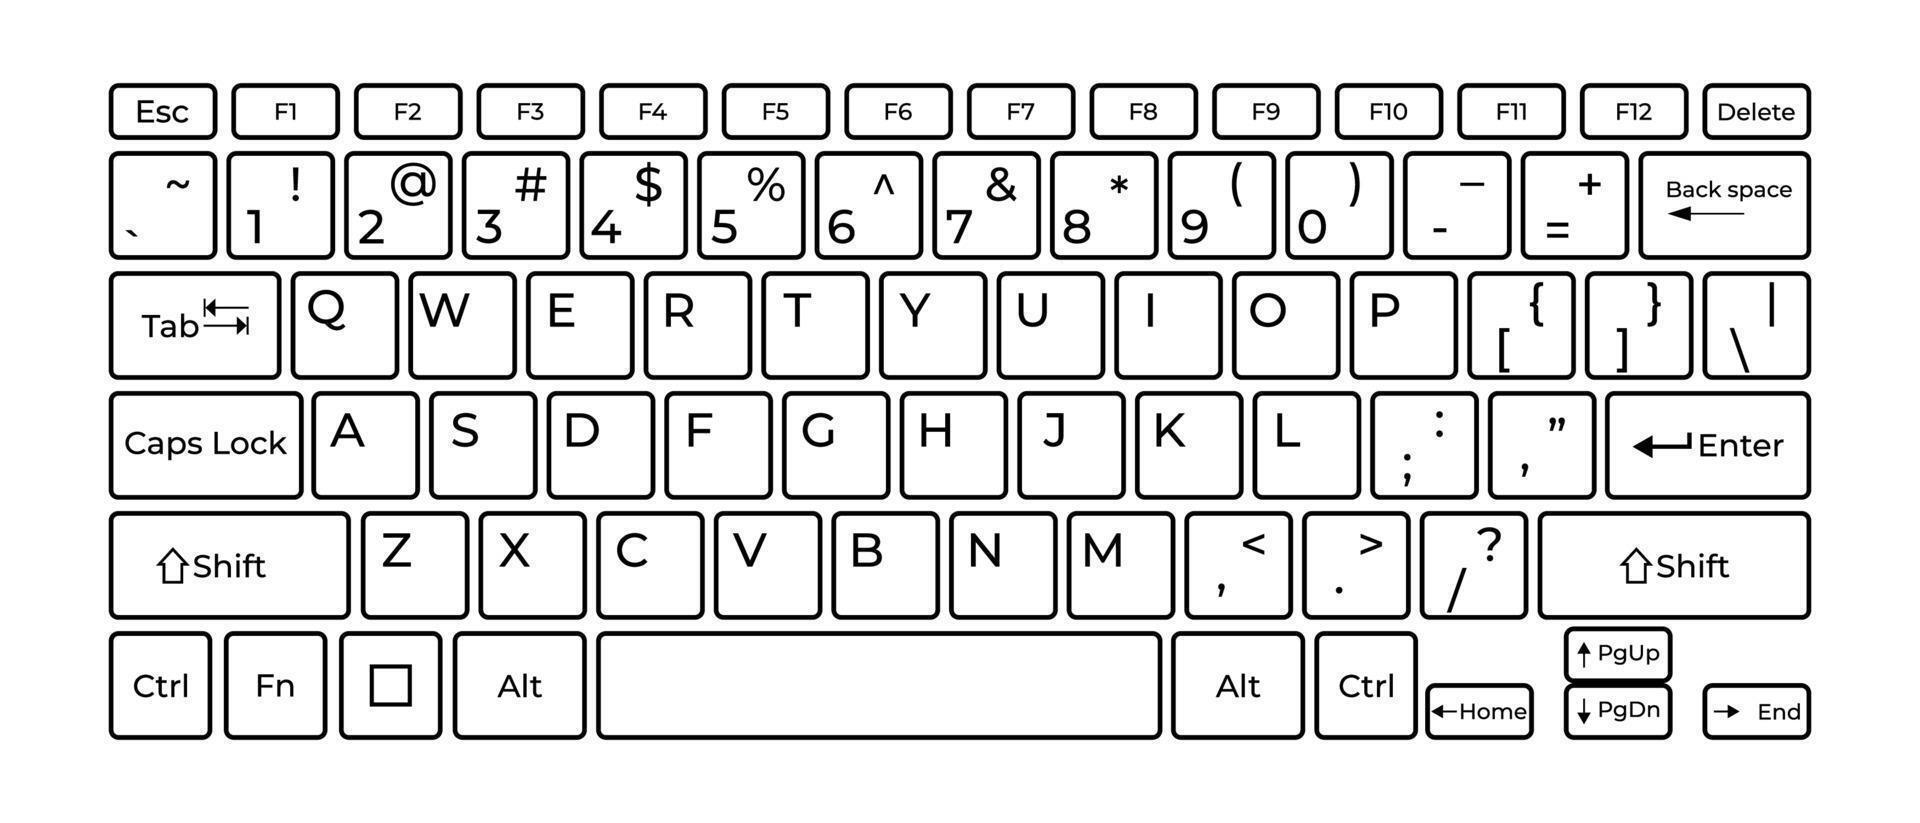
\includegraphics[width=0.7\textwidth]{Images/teclado.jpg}
    \caption{Imagen de un teclado}
    \label{fig:teclado}
\end{figure}
\subsection{Plataforma de despliegue}
Para el despliegue de este programa usaremos un ordenador, en el cual tengamos el contendor de \textit{Docker} instalado y encendido, y también por último, que tenga la \textit{JDK 21}, instalada, además de que este
despliegue ocurrirá en un sistema Windows primero, y después se barajará la posibilidad de desplegarlo en sistemas \textit{Linux}, basados en \textit{Debian}.
\clearpage
\subsection{Arquitectura logica}
Estructura del proyecto en el diagrama de clases:
\subsubsection{Diagrama de clases}
% metemos la imagen de la carpeta images que se llama diagrama.png
\begin{figure}[ht]
    \centering
    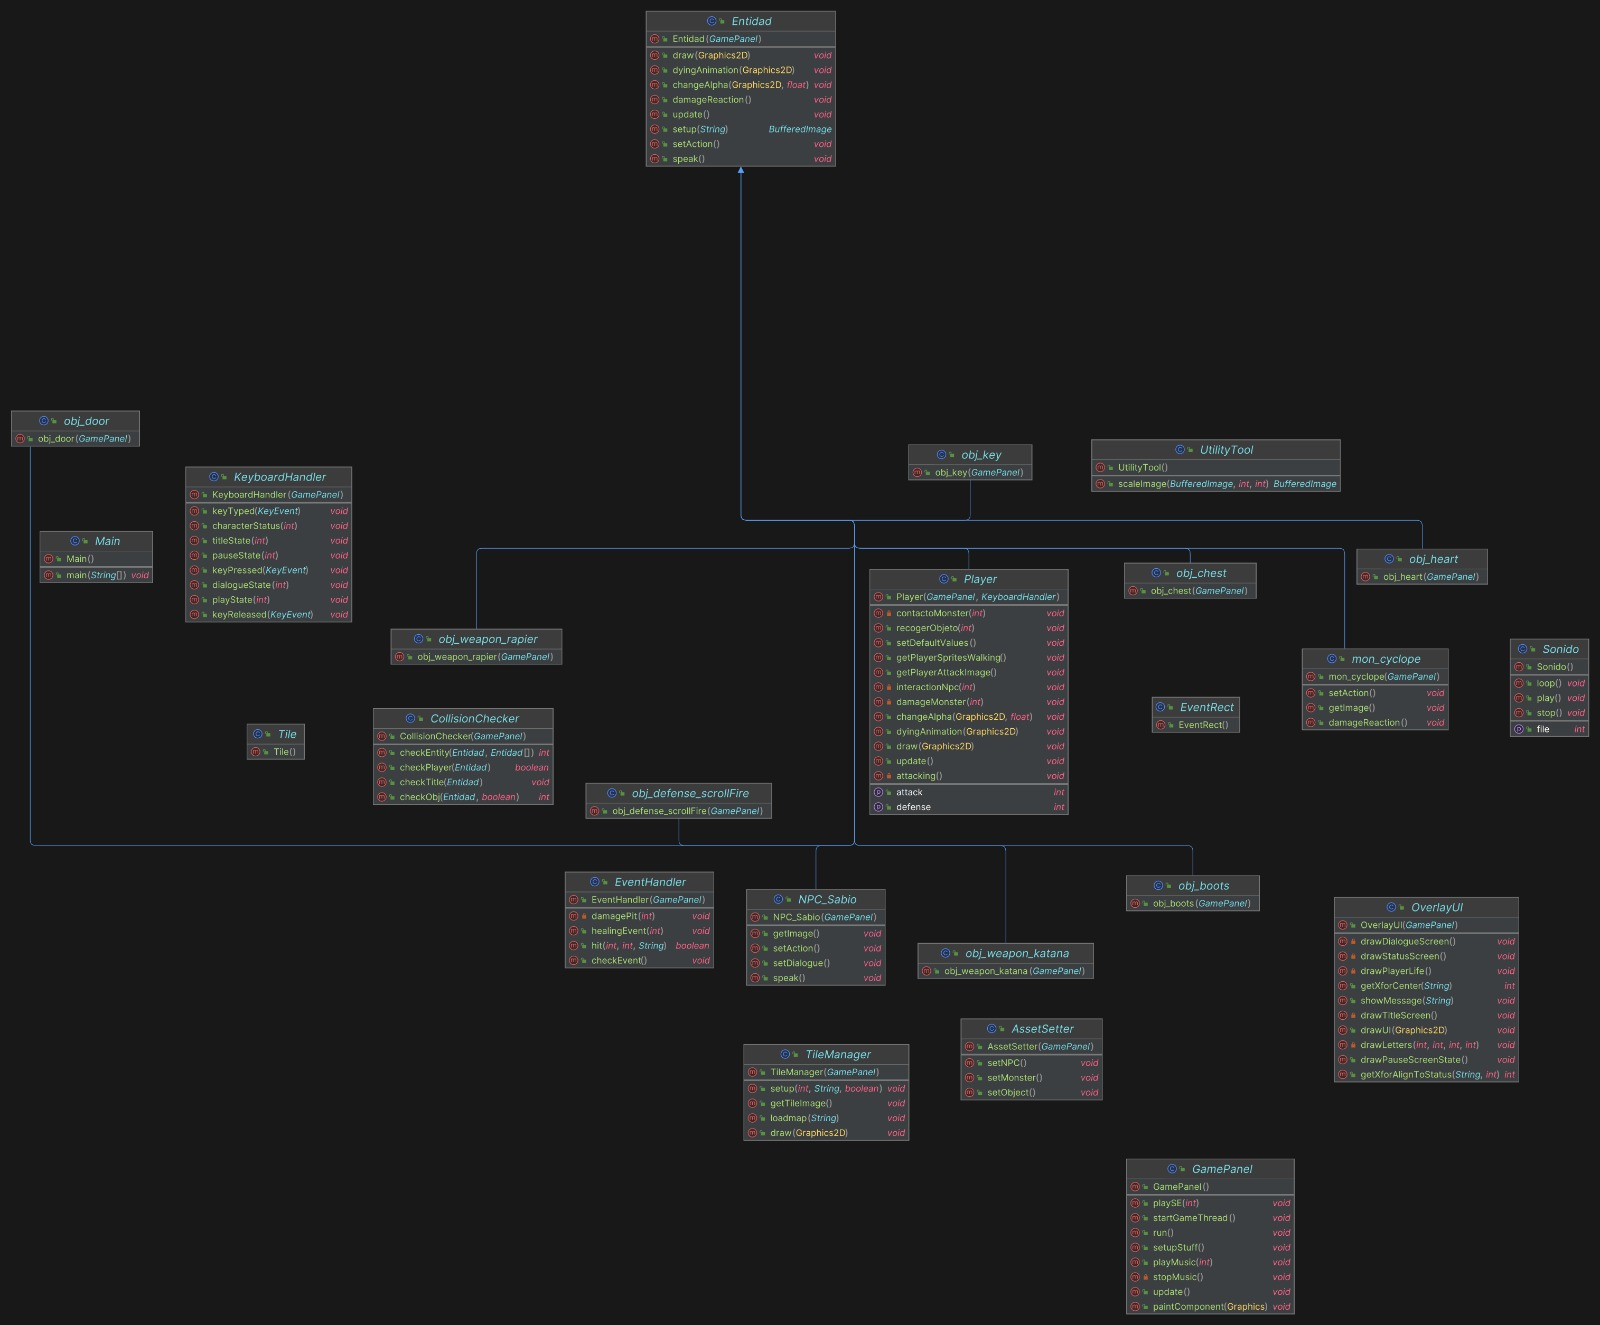
\includegraphics[width=0.7\textwidth]{Images/diagrama.jpg}
    \caption{Diagrama de clases}
    \label{fig:diagrama-clases}
\end{figure}

\subsubsection{Explicaciones del diagrama}
Como podemos ver en el diagrama, hay varias clases importantes a lo largo de la estructura del mismo, que son, \textbf{Player, Gamepanel y Entidad}, estas clases son las más importantes ya que
nos ayudan a definir muchas cosas.\\
En el caso de \textit{Entidad}, nos permite desarrollar enemigos, objetos, npc y el propio jugador, ya que estos objetos, extienden de \textit{Entidad}, lo que deja que esta clase sea una clase llena de atributos.
\subsubsection{Metodo run}
En cuanto a \textit{Gamepanel}, esta clase sería la encargada de tener el panel de juego y conectarse con todas las clases del proyecto, ya que, por ejemplo define
el tamaño de los assetts, el tamaño del texto, y varios aspectos más de dentro del juego, esta clase además es de las más importantes ya que contiene parte de los métodos más críticos del proyecto como por ejemplo el siguiente.\\
\begin{figure}[ht]
    \centering
    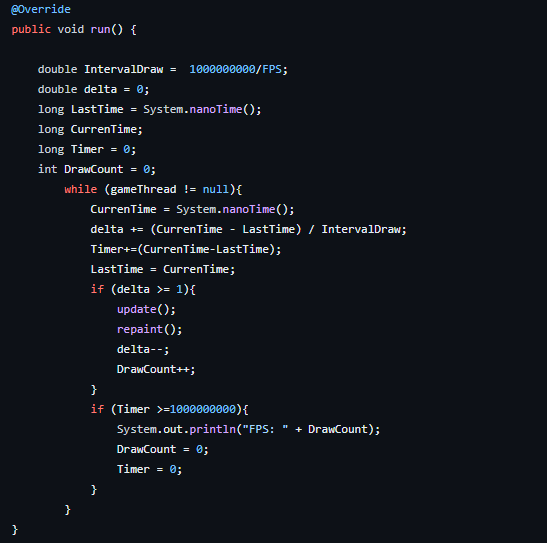
\includegraphics[width=0.7\textwidth]{Images/fpsMethod.PNG}
    \caption{Método del hilo principal}
    \label{fig:metodos}
\end{figure}
\\
Este método empieza inicializando 6 variables que le servirán para calcular un \textit{delta}, para ello hace uso de esta ecuación:
$$\text{IntervalDraw} = \frac{1}{\text{FPS}}$$
Como vemos esta ecuación sería la inversa de los \textit{FPS o Frames per Second}, dicho esto explicaremos cada variable.
\begin{itemize}
    \item \textit{IntervalDraw:} esta variable es la encargada de calcular en nanosegundos el tiempo necesario para dibujar un fotograma a la velocidad deseada
    \item \textit{delta:} Lleva un seguimiento del tiempo transcurrido desde el último fotograma.
    \item \textit{LastTime:} Almacena el tiempo en nanosegundos en el que se procesó el último fotograma.
    \item \textit{CurrenTime:} Almacena el tiempo actual en nanosegundos.
    \item \textit{Timer:} Lleva el seguimiento del tiempo transcurrido.
    \item \textit{DrawCount:} Es el contador de FPS del juego.
\end{itemize}
\textbf{Bucle principal}\\
Esta parte del codigo, ejecuta un bucle (El bucle se ejecuta mientras gameThread no sea nulo (es decir, mientras el juego esté funcionando)) en el cual ocurre lo siguiente:
\begin{itemize}
    \item Se actualiza el valor de CurrenTime.
    \item Se calcula el tiempo transcurrido desde el último fotograma y se agrega a delta.
    \item Se actualiza el valor de LastTime.
    \item Si delta supera 1, se llama a los métodos update() y repaint() para actualizar y dibujar el siguiente fotograma.
    \item Se decrementa delta en 1 y se incrementa DrawCount.
    \item Si Timer supera 1 segundo (1,000,000,000 nanosegundos), se muestra el número de fotogramas dibujados en la consola y se reinician los contadores.
\end{itemize}
Es decir, este metodo controla la lógica del dibujado o render del juego para que sea siempre de 60 fotogramas por segundo, es decir, dibuja 60 veces por segundo lo que tenemos en pantalla
de esta manera no tenemos valores extremadamente altos que no sirve de nada tener en un juego de este estilo, ya que no necesitamos que se dibuje todo 300 mil veces por segundo.\\
Acabando con las clases principales, tenemos la clase \textit{Player} la cual tiene todos los métodos relacionados al jugador, es decir, el método de atacar, el método de moverse, colisiones con objetos,
etc \dots
\clearpage
\subsubsection{Método loadmap}
Aun asi, vale la pena destacar varios métodos interesantes como el de \textit{"loadmap"}, que encontramos en la clase \textit{"TileMananger"}, la clase encargada de leer el mapa del juego.
\begin{figure}[ht]
    \centering
    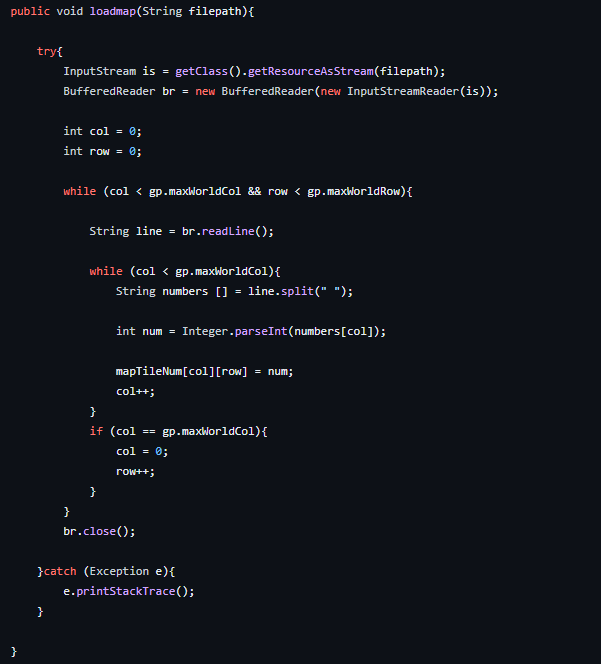
\includegraphics[width=0.7\textwidth]{Images/loadmap.PNG}
    \caption{Método de carga de mapas}
    \label{fig:metodos}
\end{figure}
\\
\textbf{Explicacion del metodo}\\
Este método funciona de la siguiente manera, a modo de resumen, lee el archivo .txt del mapa que esta compuesto solo de números y a cada número le asigna una casilla, de esta manera, según el número la casilla
tiene una imagen u otra.\\
Ahora de forma extensa, explicaremos paso por paso que hace este método:
\begin{enumerate}
    \item \texttt{El método toma una cadena, \textit{"filepath"}, esta cadena se refiere a la ubicación del mapa en el sistema de archivos del ordenador, es decir, la ruta del archivo}
    \item \texttt{"InputStream is = getClass().getResourceAsStream(filepath); BufferedReader br = new BufferedReader(new InputStreamReader(is));" esta parte del codigo lo que hace es crear un BufferReader que lee el archivo del mapa.}
    \item \texttt{"getClass().getResourceAsStream(filepath)" lo que hace es localizar el archivo en el sistema.}
    \item \texttt{Las variables \textit{row} y \textit{col} nos sirven para saber en que posición del mapa se encuentra.}
    \item \texttt{"while (col < gp.maxWorldCol \&\& row < gp.maxWorldRow)" el bucle continua mientras no se llegue al final del mapa}
    \item \texttt{"String line = br.readLine();" simplemente lee una linea del archivo}
    \item \texttt{"while (col < gp.maxWorldCol)" el bucle se ejecuta para cada columna actual}
    \item \texttt{"String numbers [] = line.split(" "); int num = Integer.parseInt(numbers[col]); mapTileNum[col][row] = num; col++;" aquí se divide la línea en números, se convierte cada número a un entero y se almacena en el array \textit{mapTileNum}}
    \item \texttt{"if (col == gp.maxWorldCol){ col = 0; row++; }" Cuando se ha llegado al final de una fila, se incrementa la variable \textit{row} y se reinicia la variable \textit{col}}
    \item \texttt{"br.close();" cierra el BufferReader.}
    \item \texttt{Y por ultimo el catch captura la excepcion en caso de que se produzca}
\end{enumerate}
Este es un método muy curioso ya que puede producir otra excepción más que no he controlado, estamos hablando de la famosa excepción \textit{java.lang.OutOfMemoryError}, debido a que si tenemos un mapa muy grande
la máquina virtual de java, \textit{JVM} se queda sin memoria en el heap y detiene el programa porque ha "roto".
\clearpage
\subsubsection{Método draw}
Otro método interesante sería el método \textit{"draw"} de nuevo de la clase \textit{"TileMananger"}, el cual se encarga de dibujar las "casillas" de juego.\\
De forma resumida, va dibujando las casillas en la posición determinada en el mapa del juego.\\
\textbf{Explicación del método}\\
Este método es bastante simple de entender si hemos entendido los anteriores, por lo que procederemos a su desglose:
\begin{enumerate}
    \item \texttt{"public void draw(Graphics2D g2)" primero recibe un objeto del tipo Graphics2D como argumento que usará para dibujar en pantalla.}
    \item \texttt{"worlCol y worlRow" son las variables que usaremos para rastrear la posición en la que nos encontramos}
    \item \texttt{"while(Wordlcol < gp.maxWorldCol \&\& WorldRow < gp.maxWorldRow)" este bucle continua mientras no lleguemos al final del mapa}
    \item \texttt{"int tileNum = mapTileNum[Wordlcol][WorldRow]" y aqui obtenemos el número de la casilla que se va a dibujar}
    \item \texttt{int worldX = Wordlcol * gp.tileSize; int worldy = WorldRow * gp.tileSize} aquí calculamos las coordenadas \texttt{x} e \texttt{y} del juego
    \item \texttt{"int screenX = worldX - gp.player.wordlx + gp.player.ScreenX; int screenY = worldy - gp.player.wordly + gp.player.ScreenY" aqui se calculan las coordenadas de la pantalla}
    \item \texttt{"g2.drawImage(tile[tileNum].image,screenX,screenY, null);" aqui dibujamos la casilla}
    \item \texttt{Incrementamos las columnas de la variable que rastrea las columnas}
    \item \texttt{"if (Wordlcol == gp.maxWorldCol){ Wordlcol = 0; WorldRow++; }" cuando se ha llegado al final de una fila, se incrementa la variable WorldRow y se reinicia la variable Wordlcol}
\end{enumerate}
\begin{figure}[ht]
    \centering
    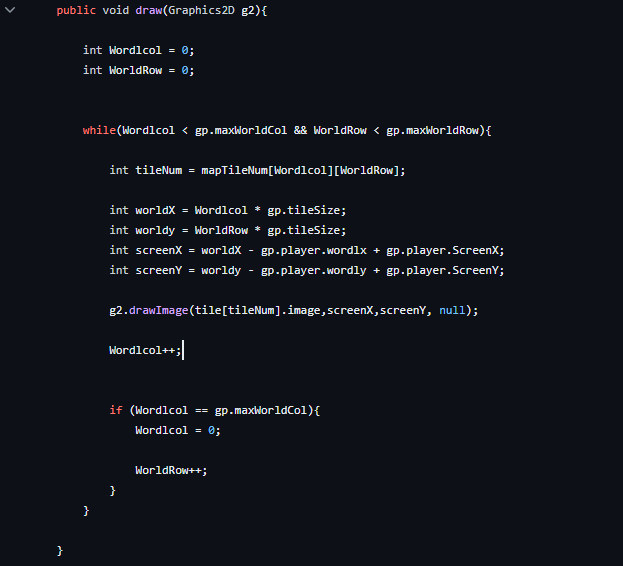
\includegraphics[width=0.6\textwidth]{Images/draw.PNG}
    \caption{Método de dibujado de mapas}
    \label{fig:metodos}
\end{figure}


\clearpage
% ------------------------------------------------
\subsection{Diagrama de casos de uso}
En el diagrama de casos de uso, tenemos un actor que seria el jugador. Este actor realizaría varias funciones, como por ejemplo:
\begin{itemize}
    \item Crear una partida
    \item Cargar una partida
    \item Empezar el juego
    \item Mover el personaje
    \item Pausar el juego
    \item Ver el estado del personaje
    \item Salir del juego
    \item Activar eventos
    \item Combatir
    \item Interactuar con NPCs
    \item Obtener objetos, experiencia, dinero.
    \item Comprar y Vender objetos
    \item Interactuar con el entorno
\end{itemize}

\begin{figure}[ht]
    \centering
    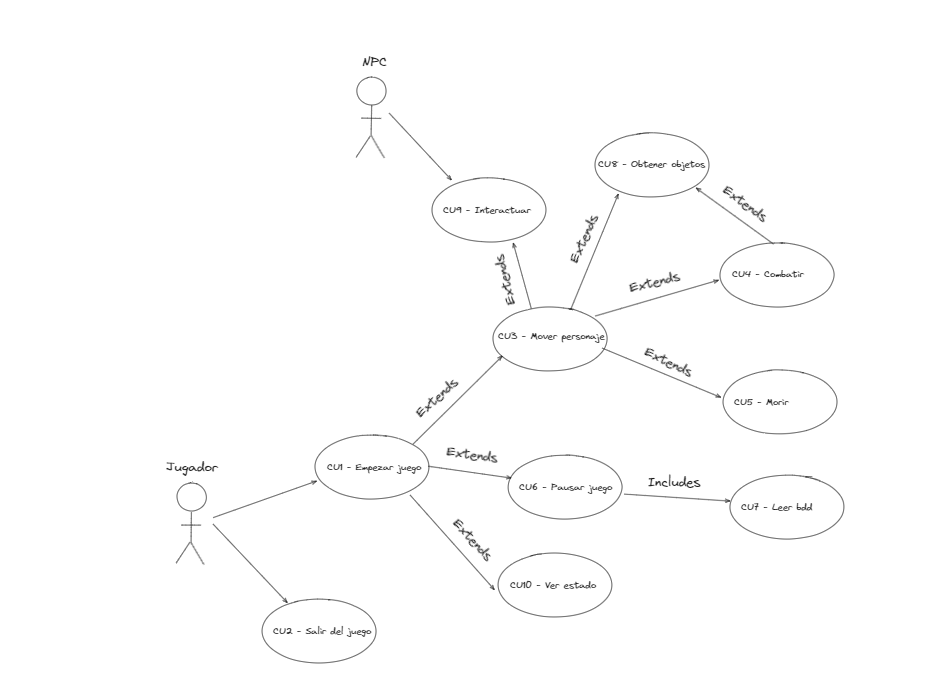
\includegraphics[width=0.6\textwidth]{Images/diagramaCU.PNG}
    \caption{Diagrama de casos de uso}
    \label{fig:diagramas}
\end{figure}

\clearpage
% -----------------------------------------------

\begin{table}[ht]
    \centering
    \begin{tabular}{|c|p{14cm}|} 
        \hline
        \textbf{Apartados}       & \textbf{CU1-Crear partida} \\
        \hline
        Actor                    & Jugador \\
        \hline
        Descripción              & El jugador selecciona en la pantalla del menú principal la opción de crear una partida nueva, lo que provoca la creación de un nuevo archivo de guardado \\
        \hline
        Frecuencia de uso        & Baja \\
        \hline
    \end{tabular}
    \caption{Caso de uso 1 - Crear partida}
    \label{tab:casosdeuso-table}
\end{table}

\begin{table}[ht]
    \centering
    \begin{tabular}{|c|p{14cm}|} 
        \hline
        \textbf{Apartados}       & \textbf{CU2-Cargar partida} \\
        \hline
        Actor                    & Jugador \\
        \hline
        Descripción              & El jugador selecciona en la pantalla del menú principal la opción de cargar una partida, lo que provoca la lectura de un archivo de guardado existente \\
        \hline
        Frecuencia de uso        & Baja \\
        \hline
    \end{tabular}
    \caption{Caso de uso 2 - Cargar partida}
    \label{tab:casosdeuso-table}
\end{table}

\begin{table}[ht]
    \centering
    \begin{tabular}{|c|p{14cm}|} 
        \hline
        \textbf{Apartados}       & \textbf{CU3-Mover personaje} \\
        \hline
        Actor                    & Jugador \\
        \hline
        Descripción              & El jugador por medio de las teclas mueve el personaje en pantalla en cualquiera de las 4 direcciones \\
        \hline
        Frecuencia de uso        & Alta \\
        \hline
    \end{tabular}
    \caption{Caso de uso 3 - Mover personaje}
    \label{tab:casosdeuso-table}
\end{table}

\begin{table}[ht]
    \centering
    \begin{tabular}{|c|p{14cm}|} 
        \hline
        \textbf{Apartados}       & \textbf{CU4-Obtener cosas} \\
        \hline
        Actor                    & Jugador \\
        \hline
        Descripción              & El jugador obtiene bien sean objetos, monedas o experiencia durante el tiempo de juego \\
        \hline
        Frecuencia de uso        & Media \\
        \hline
    \end{tabular}
    \caption{Caso de uso 4 - Obtener cosas}
    \label{tab:casosdeuso-table}
\end{table}

\begin{table}[ht]
    \centering
    \begin{tabular}{|c|p{14cm}|} 
        \hline
        \textbf{Apartados}       & \textbf{CU5-Pausar el juego} \\
        \hline
        Actor                    & Jugador \\
        \hline
        Descripción              & El jugador presiona la tecla "P" que pausa el juego totalmente, es decir, el juego queda totalmente congelado hasta que vuelva a pulsar la tecla "P" de nuevo \\
        \hline
        Frecuencia de uso        & Baja \\
        \hline
    \end{tabular}
    \caption{Caso de uso 5 - Pausar el juego}
    \label{tab:casosdeuso-table}
\end{table}

\begin{table}[ht]
    \centering
    \begin{tabular}{|c|p{14cm}|} 
        \hline
        \textbf{Apartados}       & \textbf{CU6-Interactuar} \\
        \hline
        Actor                    & Jugador \\
        \hline
        Descripción              & El jugador hablaría, chocaría o tocaría algun personaje o elemento del entorno del juego \\
        \hline
        Frecuencia de uso        & Alta \\
        \hline
    \end{tabular}
    \caption{Caso de uso 6 - Interactuar}
    \label{tab:casosdeuso-table}
\end{table}

\begin{table}[ht]
    \centering
    \begin{tabular}{|c|p{14cm}|} 
        \hline
        \textbf{Apartados}       & \textbf{CU7-Comprar} \\
        \hline
        Actor                    & Jugador \\
        \hline
        Descripción              & El jugador al realizar el caso de uso 6 "CU6", puede que interactue con un mercader, en este caso, puede comprar o vender, vender seria el "CU8" \\
        \hline
        Frecuencia de uso        & Baja \\
        \hline
    \end{tabular}
    \caption{Caso de uso 7 - Comprar}
    \label{tab:casosdeuso-table}
\end{table}

\begin{table}[ht]
    \centering
    \begin{tabular}{|c|p{14cm}|} 
        \hline
        \textbf{Apartados}       & \textbf{CU8-Vender} \\
        \hline
        Actor                    & Jugador \\
        \hline
        Descripción              & El jugador selecciona en la pantalla de inventario un objeto, lo que provoca la eliminación de una existencia de ese objeto en concreto o la resta en una o varias unidades las existencias del objeto a cambio de monedas \\
        \hline
        Frecuencia de uso        & Baja \\
        \hline
    \end{tabular}
    \caption{Caso de uso 8 - Vender}
    \label{tab:casosdeuso-table}
\end{table}

\begin{table}[ht]
    \centering
    \begin{tabular}{|c|p{14cm}|} 
        \hline
        \textbf{Apartados}       & \textbf{CU9-Empezar el juego} \\
        \hline
        Actor                    & Jugador \\
        \hline
        Descripción              & El jugador despues de realizar el CU1 o bien el CU2, realizaría esta acción \\
        \hline
        Frecuencia de uso        & Alta \\
        \hline
    \end{tabular}
    \caption{Caso de uso 9 - Empezar juego}
    \label{tab:casosdeuso-table}
\end{table}

\begin{table}[ht]
    \centering
    \begin{tabular}{|c|p{14cm}|} 
        \hline
        \textbf{Apartados}       & \textbf{CU10-Ver estado} \\
        \hline
        Actor                    & Jugador \\
        \hline
        Descripción              & El jugador presiona la tecla "C" despues de econtrarse dentro del CU9, y se le despliega una ventana nueva en la que aparecen las estadisticas de su personaje \\
        \hline
        Frecuencia de uso        & Media \\
        \hline
    \end{tabular}
    \caption{Caso de uso 10 - Ver estado}
    \label{tab:casosdeuso-table}
\end{table}

\begin{table}[ht]
    \centering
    \begin{tabular}{|c|p{14cm}|} 
        \hline
        \textbf{Apartados}       & \textbf{CU11-Combatir} \\
        \hline
        Actor                    & Jugador \\
        \hline
        Descripción              & El jugador estando en el CU9, puede realizar el CU6 y despues combatir, es decir intercambiar daño con un enemigo, por medio de sus armas \\
        \hline
        Frecuencia de uso        & Media \\
        \hline
    \end{tabular}
    \caption{Caso de uso 11 - Combatir}
    \label{tab:casosdeuso-table}
\end{table}

\clearpage
\subsection{Historia del videojuego}
En esta parte explicaremos la breve narrativa, con la que cuenta el videojuego, tampoco hemos intentado hacer una narrativa super profunda, ya que requeriría de muchos más elementos
los cuales por falta de tiempo no podríamos añadir.\\
El videojuego transcurre en una época medieval, dentro de un mundo de fantasía, Eldoria, dentro de este mundo existe una gema que es capaz de realizar muchas acciones divinas, por ejemplo
curar enfermedades, provocar lluvia, otorgar suerte a una persona u entidad, etc \dots \\
Dentro del mundo hace relativamente poco, esta piedra mágica se ha perdido, y ahí es donde entra nuestro protagonista, el \textit{Ninja Rojo}, el cual se encargará de buscarla, ya que
si acaba en las manos equivocadas, sería algo terrible, pues igual que puede servir para el bien, también concede poderes para el mal.\\
De forma resumida sería la historia planeada para el videojuego, cabe destacar que por ejemplo una propuesta de mejora, sería ampliar este apartado algo más, meter más personajes, etc \dots

\clearpage

% -------------------------------------------------
\subsection{Pantallas del juego}
Dentro de esta sección hablaremos de las pantallas que hemos desarrollado en el juego, es decir, el menú principal, el inventario, por ejemplo.\\
Primero empezaremos con la pantalla del menú principal en la cual encontramos varios elementos.\\
Para empezar, tenemos que tener en cuenta que esta pantalla se dibuja con el método \textit{drawTitleScreen}, este método, nos permite crear la pantalla del menú. A continuación, lo primero de lo que hablaremos es la imagen de fondo del juego, hemos optado por usar una imagen en vez de por ejemplo un color sólido, o un vídeo incluso, ya que nos parece más creativo que un color, pero más sencillo que un vídeo, tambén algo que cabe destacar es que hay otra imagen, en este caso del protagonista, hemos optado por poner al protagonista, ya que no hemos
desarrollado ningún icono para el juego y por ejemplo, podríamos poner el icono que usamos dentro de la ventana main. Por otra parte, lo que tenemos son las letras, estas letras vienen hechas de la clase OverlayUI, la cual se encarga de estas características, también si nos fijamos, tenemos una especie de cursor, el cual nos permite seleccionar una opción de menú, esto se ve referenciado en el código referente a la lógica del menú principal.\\
Dentro de esta pantalla no hay mucho que podamos hacer, es decir, fuera de elegir si queremos jugar, crear partida o salir del juego, no hay mucho más que se pueda hacer.\\

La segunda pantalla a analizar es la pantalla de juego, en ella transcurse todo el programa realmente, tenemos un panel que sigue al jugador allá donde vaya, y que nos muestra los enemigos, npc y casillas del mapa, esta pantalla además cuenta con una variación que es la pantalla con inventario, esta pantalla nos muestra al lado izquierdo las estadísticas del jugador, y a otro lado el inventario del mismo con descripciones para cada objeto.
Por otro lado, dentro de esta pantalla también observamos los corazones de vida del jugador. Y por último, la pantalla de pausa que simplemente es un cuadro con la palabra Pausa.


\clearpage
% -------------------------------------------------



\section{Desarrollo realizado}
Para el desarrollo del proyecto hemos usado las siguientes herramientas:
\begin{itemize}
    \item IntelliJ
    \item Docker
    \item Jooq
    \item JDK 21
    \item Visual studio Code
    \item \LaTeX
    \item Excalidraw
    \item Github Repositories
    \item MySQL
\end{itemize}
Ahora pasaremos a explicar el código de una manera más detallada, parándonos un poco más clase por clase para explicar lo que hemos desarrollado.
\subsection{Detalles del codigo desarrollado}
Empezaremos describiendo lo que realiza la clase principal, la clase \textit{"Main"}, cuyo código es:
\begin{lstlisting}
    package main;

import javax.swing.*;
import java.awt.*;

public class Main {
    public static void main(String args[]){
        JFrame win = new JFrame();
        win.setDefaultCloseOperation(JFrame.EXIT_ON_CLOSE);
        win.setResizable(false);
        //win.setBackground(Color.black);
        win.setTitle("Eldoria");

        GamePanel gpanel = new GamePanel();
        win.add(gpanel);

        win.pack();

        win.setLocationRelativeTo(null);
        win.setVisible(true);
        gpanel.setupStuff();
        gpanel.startGameThread();

    }
}
\end{lstlisting}
% ----Cambiar por el tema de full screen------
Dentro de este código encontramos varios aspectos a destacar, el primero es que estamos creando un JFrame en primera instancia y luego le estamos diciendo tambien que al darle a la "X", nos cierre el programa automaticamente.
Continuamos diciéndole que no queremos un resize de la ventana actual del juego, por eso el false, seguimos con el titulo, y a continuacion la instancia de GamePanel, la cual nos servirá para instanciar más cosas.
Centramos la ventana con el setLocationRelativeTo, la hacemos visible y le decimos a GamePanel que vaya dibujando ciertas cosas del videojuego e inicie el hilo principal del juego.\\

Continuamos la explicación con la clase \textit{"Gamepanel"}, la cual es la encargada de realizar varias acciones principales dentro de la aplicación, si bien es cierto que hemos explicado algún método ya, explicaremos el resto
que no son tan importantes pero igualmente son interesantes de saber.\\
\begin{lstlisting}
    public void setupStuff(){
        aSetter.setObject();
        aSetter.setNPC();
        aSetter.setMonster();
        playMusic(1);
        gameState = titleState;
    }
\end{lstlisting}
Este método es el que se encarga de poner todo a punto en el \textit{"tablero de juego"}, como vemos, llama al metodo setObject, setNpc, setMonster, y playMusic, los cuales se encargan respectivamente
de poner los objetos en el mapa, los npc, los monstruos y reproducir la música de fondo, por último se cambia la variable de gamestate que es con la que se jugará dentro del código para poner el juego en pausa, o
en el menú principal, por ejemplo.\\
Continuamos con un método que actualmente no es de está manera pero aun así es interesante de ver ya que ha servido de base para futuras versiones, y es el método paintComponent antes de realizar la función de tener el juego
en pantalla completa:
\begin{lstlisting}
    public void paintComponent(Graphics g){

    super.paintComponents(g);
    Graphics2D g2 = (Graphics2D)g;
    g2.setColor(Color.BLACK);
    g2.fillRect(0, 0, getWidth(), getHeight());

    //Title screen
    if (gameState == titleState){
        overlayUI.drawUI(g2);
    }
    //Others
    else {
        ///casillas
        TileM.draw(g2);
        //Adicion de entidades a la lista
        entidadList.add(player);
        for (int i = 0; i<npc.length; i++){
            if (npc[i] != null){
                entidadList.add(npc[i]);
            }
        }
        for (int i=0; i<obj.length; i++){
            if (obj[i]!= null){
                entidadList.add(obj[i]);
            }
        }
        for (int i=0; i<monster.length; i++){
            if (monster[i]!= null){
                entidadList.add(monster[i]);
            }
        }
        /// ordenado
        Collections.sort(entidadList, new Comparator<Entidad>() {
            @Override
            public int compare(Entidad o1, Entidad o2) {
                int result = Integer.compare(o1.wordly, o2.wordlx);
                return 0;
            }
        });

        //Draw entity
        for (int i = 0; i<entidadList.size(); i++ ){
            entidadList.get(i).draw(g2);
        }

        /// Empty entity list
        entidadList.clear();


        //Overlay UI
        overlayUI.drawUI(g2);

    }
    g2.dispose();
}
\end{lstlisting}
Para empezar, este método sería el encargado de pintar todos los componentes en la pantalla, es decir, pinta las casillas y el fondo del juego sobre el que se pondrán las imágenes usadas para el juego,
también se encarga de dibujar o renderizar, los monstruos, npcs, y el personaje. Profundizaremos más en ello.\\
Lo primero que realiza, después de coger los 4 parámetros que coge, es cerciorarse del gameState en el que nos encontramos, al hacerlo dibujará la pantalla de título o la de juego, en caso de estar en la
de titulo, lo que encontramos es una llamada a la clase encargada de la \textit{User Interface}, la hemos llamado \textit{OverlayUI}, ya que no deja de ser lo que se conoce tipicamente en imagen como overlay,
y UI debido a que se trata de la interfaz de usuario. Si seguimos, en caso de no estar en el estado de pantalla de titulo, lo que haría el código es seguir por la parte del \textit{else}, en este parte el código empieza
dibujando las casillas con el ".draw", y continua añadiendo las entidades al juego, en este programa como todas las entidades las guardamos en listas, tenemos que realizar un bucle for que nos permita recorrer la lista
que contiene las entidades. Al acabar llegamos a la parte que ordena las entidades con la interfaz \textit{Comparator}, sobreescribimos el método de esta interfaz para ordenadr las entidades y continuamos con el código.
Una vez que tenemos ordenadas las entidades, lo que hará el código es dibujar las propias entidades, ordenadas en función de donde aparece el jugador, cuanto más cerca más prioridad tiene de ser dibujada la entidad.
por último limpiamos la lista de entidades \textit{temporales} y con todo puesto, le decimos a la clase del Overlay, que lo dibuje todo, y para acabar, metemos un .dispose, para acabar. \\
Antes de realizar la funcionalidad de tener el juego en pantalla completa, se realizaba el dibujado de esa manera, actualmente, seguimos usando el mismo método salvo que cuenta con una variación, la cual es que hemos eliminado,
varias instancias de g2, es decir del objeto de Graphics2D, esto es debido a que para mostrar el juego en la pantalla completa el juego lo que realiza es lo siguiente:\\
\begin{figure}[ht]
    \centering
    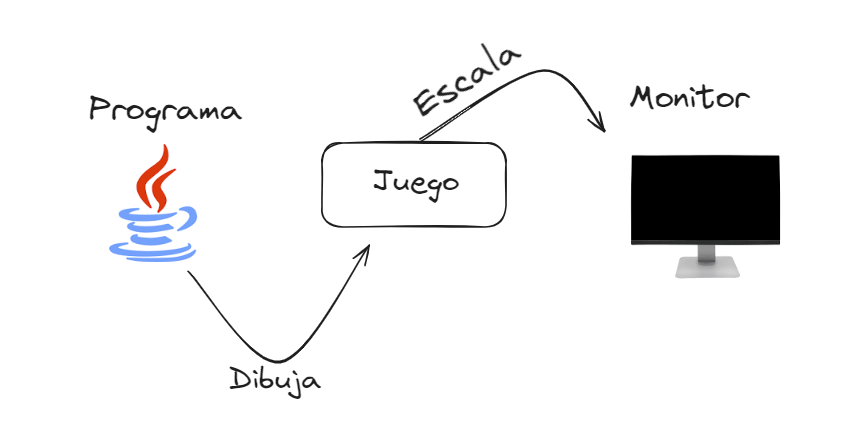
\includegraphics[width=0.6\textwidth]{Images/Fullscrennmode.PNG}
    \caption{¿Cómo dibuja el programa la pantalla completa?}
    \label{fig:fullscreen}
\end{figure}
Esto es importante tenerlo en cuenta ya que después de ser dibujado el juego, necesita ser escalado a la resolución de nuestro monitor, en las primeras fases del desarrollo, se realizó el juego en un formato de 4:3,
formato clásico de monitores más bien modestos o antiguos, según se implementó la función de pantalla completa, se ha tenido que cambiar lo que se conoce como \textit{aspect ratio} a uno más actual y más usado, como puede
ser el formato de 16:9, algo más estirado que el clásico 4:3, esto permite que se pueda mostrar el juego en monitores de 1920x1080 pixeles, o tambien en monitores 4K, de resolución 3840x2160 pixeles. ¿Por qué es importante saber esto?
esto es crucial, ya que a la hora de desarrollar las interfaces del juego como son el menú principal, la pantalla de estado del personaje, mensajes en pantalla y demás interfaces que puedan salir dentro del juego, necesitamos en su
mayoría, escalarlas al tamaño de la pantalla en la que se muestra, ya que, de lo contrario podríamos encontrar fallos visuales en el juego, como dialogos mal puestos, interfaces que se salen de la pantalla, que están posicionadas mal, por ejemplo \dots \\


\clearpage
% -----------------------------------

Por ejemplo vamos a echar un vistazo a otra clase interesante del proyecto la cual es \textit{KeyboardHandler}, esta clase se ocupa de registrar las pulsaciones del teclado y realizar las acciones en función de la tecla
presionada. Vamos a analizar el método que se encarga del movimiento del personaje.
\begin{lstlisting}
    @Override
    public void keyPressed(KeyEvent e) {
        int code = e.getKeyCode();
        //Title state
        if (gp.gameState == gp.titleState){
            titleState(code);
        }
        ///Play state
        else if (gp.gameState == gp.playState){
            playState(code);
        }
        ///Pause State
        else if (gp.gameState == gp.pauseState){
            pauseState(code);
        }
        ///Dialogue state
        else if (gp.gameState == gp.dialogueState){
            dialogueState(code);
        }
        /// Status state
        else if (gp.gameState == gp.statusState){
            characterStatus(code);
        }
    }
\end{lstlisting}

Como vemos este método tiene varias partes y estados haciendo referencia al \textit{GameState}, por lo que nosotros primeramente nos fijaremos en el \textit{playstate}, el cual contiene la lógica para mover el personaje.
\begin{lstlisting}
    public void playState(int code){
        if (code == KeyEvent.VK_W){
            upPressed = true;
        }
        if (code == KeyEvent.VK_A){
            leftPressed = true;
        }
        if (code == KeyEvent.VK_S){
            downPreseed = true;
        }
        if (code == KeyEvent.VK_D){
            rightPressed = true;
        }
        if (code == KeyEvent.VK_P){
            if (gp.gameState == gp.playState){
                gp.gameState = gp.pauseState;
            }else if (gp.gameState == gp.pauseState){
                gp.gameState = gp.playState;
            }

        }
        if (code == KeyEvent.VK_C){
            gp.gameState = gp.statusState;
        }
        if (code == KeyEvent.VK_ENTER){
            enterPressed = true;
        }
    }
\end{lstlisting}
Como vemos en este código, gracias a la clase \textbf{KeyEvent} de \textit{ava.awt.event.KeyEvent}, podemos reconocer la tecla pulsada con un determinado código que recibimos del input del usuario por el teclado. Esto, 
nos facilita la creación de la lógica de su movimiento, y más interacciones con el juego, debido a que cada tecla contiene un codigo que podemos poner en un switch como se ve en el código para poder mover el personaje.
Esta clase también nos sirve como hemos visto en el primer código, para poder usar otras teclas, pausar el juego, interactuar con un npc, atacar, etc \dots \\
Otro código interesante sería el que se encarga de dibujar los cuadros de dialogo.
\begin{lstlisting}
    private void drawDialogueScreen() {
        int x = gp.tileSize*2;
        int y = gp.tileSize/2;
        int width = gp.screenWidth - (gp.tileSize*4);
        int height = gp.tileSize*4;

        drawLetters(x, y, width, height);

        g2.setFont(g2.getFont().deriveFont(Font.PLAIN,26F));
        x += gp.tileSize/2;
        y += gp.tileSize;
        g2.drawString(dialogo,x,y);

        for (String line : dialogo.split("\n")){
            g2.drawString(line, x, y);
            y +=40;
        }
    }
\end{lstlisting}
Primero inicializamos variables, en este caso la x y la y, las cuales tienen los valores de las casillas del \textit{tablero de juego}, y las utiliza para colocar los elementos en pantalla. Width y Height se calculan en funcion del acnho de la pantalla y el tamaño de la casilla.
drawletters se encarga de dibujar las letras en el cuadro del dialogo, y se configura la fuente para esas letras antes de ser dibujadas, en este caso hemos usado un tamaño de 26 puntos. En cuanto al dialogo en sí, incrementamos x e y en la mitad del tamaño de la casilla, dibujamos el contenido del dialogo en las posiciones x,y, realizamos un bucle para recorrer el dialogo, con el que dividimos las nuevas
lineas con el caracter especial. Para cada linea dibujamos en las posiciones determinadas y luego aumentamos la y, en 40 unidades para añadir un pequeño interlineado. \\

Una clase bastante extensa tambien sería la clase \textit{Player}, dentro de esta clase encontramos método útiles para la gestión del jugador dentro del juego, animaciones de atacar o posicionamiento de ciertos sprites. El método que vamos a analizar, es el método correspondiente a 
el ataque del jugador, en este caso el código sería de la siguiente manera:
\begin{lstlisting}
    private void attacking() {
        spriteCounter ++;

        if (spriteCounter <= 5){
            spriteNum = 1;
        }
        if (spriteCounter > 5 && spriteCounter <= 25){
            spriteNum = 1;

            /// Guardamos coordenadas de la hitbox
            int currentWorldX = wordlx;
            int currentWorldY = wordly;
            int hitboxWidth = hitbox.width;
            int hitboxHeight = hitbox.height;
            switch (path){
                case "up": wordly -= attackHitbox.height; break;
                case "down": wordly += attackHitbox.height; break;
                case "left": wordlx -= attackHitbox.width; break;
                case "right": wordlx += attackHitbox.width; break;
            }
            hitbox.width = attackHitbox.width;
            hitbox.height = attackHitbox.height;
            int monsterIndex = gp.cChecker.checkEntity(this, gp.monster);
            damageMonster(monsterIndex);
            wordlx = currentWorldX;
            wordly = currentWorldY;
            hitbox.width = hitboxWidth;
            hitbox.height = hitboxHeight;

        }


        if (spriteCounter > 25){
            spriteNum = 1;
            spriteCounter = 0;
            attacking = false;
        }
    }
\end{lstlisting}
Este código lo primero que hace es sumar a spritecounter, esto sirve para cambiar la animación del jugador, si tuvieramos por ejemplo varios sprites de ataque, podríamos alternar entre ellos,
jugando con spritecounter. A continuación cuando entramos al segundo condicional, lo que hacemos es, primero guardar la hitbox del jugador en unas variables que iremos cambiando conforme entremos,
en la lógica, después entramos al switch que en este caso recoge como parametro la dirección en la que esta el jugador para poder crear una nueva hitbox, en este caso de ataque.
Continuamos cambiando las dimensiones de la hitbox y ahora comprobamos si esta última hitbox, ha chocado con un enemigo, en caso correcto se realizará la acción de perder vida sobre el enemigo, sino, no ocurrirá nada.
En fases tempranas del desarrollo para probar esto, se puso una traza a modo de prueba en la que salía un mensaje por consola si fallabamos el ataque, así podiamos saber si acertabamos o no.\\
\clearpage
% ----------------------------------
Hablemos de los \textit{Tiles}, en este caso tenemos dos tipos de Tiles, los colisionables y los no colisionables, un tile colisionable no nos permite pasar por encima de el, uno no colisionable, nos permite pasar
sobre el. Es por eso que en la clase Tile, tenemos el siguiente codigo.
\begin{lstlisting}
    package tiles;

import java.awt.*;
import java.awt.image.BufferedImage;

public class Tile {

    public BufferedImage image;
    public boolean colision = false;
}
\end{lstlisting}
Dentro de esta clase lo que vemos son dos atributos, la imagen, en este caso sería el asset, y un booleano que por defecto es false, este booleano es muy interesante, ya que es el encargado, de determinar si el Tile, es colisionable o no.\\
Esta clase va de la mano realmente con una clase de la que ya hemos hablado \textit{TileManager}, esta clase se encarga de posicionar y recoger las casillas del tablero de juego, y además ayuda a dibujar las mismas, por otra parte, esta clase aunque,
ya hemos hablado de ella, vamos a explicar un método más que igualmente es necesario explicar.
\begin{lstlisting}[language=Java]
    public void setup(int index, String imageName, boolean collision){
        UtilityTool uTool = new UtilityTool();

        try{
            tile[index] = new Tile();
            tile[index].image = ImageIO
                    .read(
                        getClass()
                        .getResourceAsStream("/tiles/"+ imageName +".png")
                        );
            tile[index].image = uTool
                    .scaleImage(tile[index].image, gp.tileSize, gp.tileSize);
            tile[index].colision = collision;

        }catch (IOException e){
            e.printStackTrace();
        }
    }
\end{lstlisting}
Este código lo que hace es por medio del constructor de tile, agregar imagenes y poco a poco asignarlas segun el index que le pasemos como parámetro, luego con ayuda de uTool, redimensionamos la imagen
y por último asignamos la colisión que necesitemos, en caso de necesitarla.\\
Un ejemplo de uso, seria por ejemplo:
\begin{lstlisting}
    setup(0,"001",false);
\end{lstlisting}
Como vemos en esta llamada a setup, el metodo que hemos visto, el primer parámetro seria el index, es decir, recordemos que el mapa del juego no dejan de ser números, números que en verdad, representan casillas, estas casillas estan formadas por imagenes, 
cada número del mapa, sería el index, que buscará el método setup, el segundo parámetro sería el nombre de la imagen que buscará el método, y por último, tenemos si es colisionable o no.
\clearpage
% ------------------------------------
Un método intersante dentro de OverlayUI, puede ser el método encargado de dibujar el inventario, este método, tendría la siguiente forma:
\begin{lstlisting}
    private void drawInventory() {
        int frameX = gp.tileSize * 12;
        int frameY = gp.tileSize;
        int frameWidth = gp.tileSize * 6;
        int frameHeight = gp.tileSize * 5;
        drawLetters(frameX, frameY, frameWidth, frameHeight);
        //Slots
        final int slotXStart = frameX + 20;
        final int slotYStart = frameY + 20;
        int slotX = slotXStart;
        int slotY = slotYStart;
        ///Draw player
        for (int i = 0; i<gp.player.inventory.size(); i++){
            if (gp.player.inventory.get(i) == gp.player.currentWeapon || gp.player.inventory.get(i) == gp.player.currentShield){
                g2.setColor(new Color(240, 190,90));
                g2.fillRoundRect(slotX,slotY,gp.tileSize,gp.tileSize,10,10);
            }

            g2.drawImage(gp.player.inventory.get(i).down1, slotX, slotY, null);
            slotX += gp.tileSize;
            if (slotX >= slotXStart + gp.tileSize * 5) { 
                slotX = slotXStart;
                slotY += gp.tileSize;
            }
        }

        ///Cursor
        int cursorX = slotXStart + (gp.tileSize * slotRow);
        int cursorY = slotYStart + (gp.tileSize * slotCol);
        int cursorWidth = gp.tileSize;
        int cursorHeight = gp.tileSize;

        //Data cursor
        g2.setColor(Color.white);
        g2.setStroke(new BasicStroke(3));
        g2.drawRoundRect(cursorX, cursorY, cursorWidth, cursorHeight, 10, 10);

        // Description frame
        int dFrameX = frameX;
        int dFrameY = frameY + frameHeight;
        int dFrameWidth = frameWidth;
        int dFrameHeight = gp.tileSize*3;
        drawLetters(dFrameX,dFrameY,dFrameWidth,dFrameHeight);

        int textX = dFrameX + 20;
        int textY = dFrameY + gp.tileSize;
        g2.setFont(g2.getFont().deriveFont(28F));

        int itemIndex = getIndexOfCursor();

        if (itemIndex >= 0 && itemIndex < gp.player.inventory.size()) {
            g2.drawString(gp.player.inventory.get(itemIndex).description, textX, textY);
        }

    }
\end{lstlisting}


\clearpage
% ------------------------------------
\section{Propuestas de mejora y trabajos futuros}
Dentro de esta sección vamos a nombrar ciertos apartados que se podrían añadir en una versión futura de la aplicación, y de paso, explicaremos alguna en detalle.\\
\textbf{Objetos rompibles}: empezamos con un clásico dentro de los videojuegos y son los objetos que se pueden romper, por ejemplo vasijas que oculten dinero, corazones, u otros objetos interesantes.\\
\textbf{Más personajes}: otro tema a tratar sería el número de personajes, se podría realizar algún tipo de selector de personajes o incluso una inclusión de un sistema de clases.\\
\textbf{Sistema de clases}: un clásico en los juegos de rol, sistemas de clases que en función, de cual elijamos, tendremos unas estadísticas u otra, y en un caso extremo, si escogemos un personaje mago podremos lanzar proyectiles mágicos y con un personaje como un caballero no.\\
\textbf{Jefes}: Aparte de algo obvio, como es extender más el juego, con nuevos mapas y enemigos, podemos llegar a poner Jefes, los cuales sean enemigos especiales, con ataques únicos y batallas incluso con puzzles.\\
\textbf{Misiones}: Un útlimo aspecto que podríamos meter, puede ser un sistema de misiones, en las cuales tengamos varios tipos de misiones, por ejemplo:
\begin{itemize}
    \item Misiones principales
    Misiones en las cuales se avanza en la historia principal del juego, necesarias para poder acabar el juego.
    \item Misiones secundarias
    Misiones en las que no se avanza en la historia principal, pero se hacen misiones bien más fáciles o bien más difíciles que las principales, que tengan una recompensa mayor o menor en función de la dificultad, esto nos permitiría añadir incluso mapas nuevos, enemigos opcionales y jefes opcionales incluso, así como armas secretas.
\end{itemize}
Como trabajos futuros, nos podríamos plantear conceptos actuales ya vistos como por ejemplo \textit{Stardew Valley}, este videojuego nació de la misma manera que este propio tfg, como un tfg de universidad, el autor empezó a añadir más funciones y a completarlo cada día un poquito más,
hasta que acabó convirtiéndose en un juego bastante querido por la comunidad de videojugadores, el juego se trata de un simulador de vida campesina, en el que debemos gestionar una granja que nos ha dejado nuestro abuelo, además tiene componentes RPG, como relacionarnos con npcs, y dependiendo
de nuestra relación, pues nos darán unos objetos u otros. Otro ejemplo de trabajo futuro puede ser el videojuego \textit{Forager}, este último es un videojuego basado en el \textit{farming}, por lo que dentro de este juego nuestra meta será producir de la forma más eficiente los recursos que obtengamos,
suena de primeras simple, pero en ciertos niveles la dificultad es alta.
\begin{figure}[ht]
    \centering
    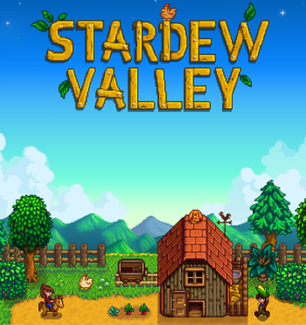
\includegraphics[width=0.3\textwidth]{Images/Logo_of_Stardew_Valley.png}
    \caption{Imagen de Stardew Valley}
    \label{fig:player}
\end{figure}
\clearpage
% ------------------------------------
\section{Bibliografia}
% ------------------------------------
\begin{itemize}
    \item \textbf{Repositorio del juego} - \url{https://github.com/Pisa-17/TFG-DAM-Eldoria/tree/main}
    \item \textbf{Excalidraw} - \url{https://excalidraw.com/}
    \item \textbf{Manual LaTeX} - \url{https://manualdelatex.com/}
    \item \textbf{Mermaid} - \url{https://mermaid.js.org/intro/getting-started.html}
    \item \textbf{IntelliJ} - \url{https://www.jetbrains.com/es-es/idea/}
    \item \textbf{Editor Pixelart} - \url{https://www.piskelapp.com/}
    \item \textbf{Como hacer Assets} - \url{https://tips.clip-studio.com/es-es/articles/2484}
    \item \textbf{TFG de la Escuela de Segovia} - \url{https://uvadoc.uva.es/bitstream/handle/10324/24495/TFG-B%201042.pdf?sequence=1}
    \item \textbf{Docker} - \url{https://www.docker.com/}
    \item \textbf{Imagen Docker MySQL} - \url{https://hub.docker.com/_/mysql/}
    \item \textbf{Out Of Memory Error} - \url{https://stackoverflow.com/questions/1596009/java-lang-outofmemoryerror-java-heap-space}
    \item \textbf{Assets} - \url{https://pixel-boy.itch.io/ninja-adventure-asset-pack}
    \item \textbf{Autor de los Assets} - \url{https://twitter.com/2Pblog1}
    \item \textbf{JooQ} - \url{https://www.jooq.org/}
    \item \textbf{Visual Studio Code} - \url{https://code.visualstudio.com/Download}
    \item \textbf{Diagrama de clases IntelliJ} - \url{https://www.jetbrains.com/help/idea/class-diagram.html}
    \item \textbf{JDK 21} - \url{https://www.oracle.com/java/technologies/javase/jdk21-archive-downloads.html}
    \item \textbf{Retro Art Article} - \url{https://medium.com/@dq_irfandi/the-nostalgia-effect-how-retro-games-influence-modern-gaming-8925be77694e}
    \item \textbf{Why retro games are so Loved?} - \url{https://www.wired.com/story/why-retro-looking-games-get-so-much-love/}
    \item \textbf{How to list code in LaTeX} - \url{https://es.overleaf.com/learn/latex/Code_listing}
    \item \textbf{Libro - The Legend of Zelda Hyrule historia} - \url{https://en.wikipedia.org/wiki/The_Legend_of_Zelda:_Hyrule_Historia} - ISBN 978-1-61655-041-7
    \item \textbf{Web para hacer Diagramas de casos de uso online} - \url{https://online.visual-paradigm.com/drive/#infoart:proj=0&dashboard}
    \item \textbf{Landing on Blasphemous - Documental} - \url{https://youtu.be/lk--if_7J9g?si=kpGDZ2x66cMYwh1K}
    \item \textbf{Python} - \url{https://www.python.org/downloads/release/python-3123/}
\end{itemize}

\clearpage
% ----------------------------------------

\begin{appendices}
    \renewcommand{\thesection}{} % Elimina la numeración de las secciones

    \section{Anexo I - Manual de Usuario}
    Los controles del juego son bastante simples, tendriamos las teclas \textit{W,A,S y D}, para mover el personaje y las teclas \textit{C, P, y ENTER} para otras acciones.
    \begin{itemize}
        \item W - Mover el personaje hacia arriba
        \item A - Mover el personaje a la izquierda
        \item D - Mover el personaje a la derecha
        \item S - Mover el personaje hacia abajo
        \item C - Ver las estadisticas del personaje
        \item P - Abrir el menu de Pausa
        \item ENTER - Interactuar con NPCs, atacar, aceptar o continuar.
    \end{itemize}
    \clearpage
    % ---------------------------------------

    \section{Anexo II - Assets}
    Para las Assets del tfg hemos usado el siguiente paquete de assets: \\
    \url{https://pixel-boy.itch.io/ninja-adventure-asset-pack} \\
    Este paquete se puede descargar de forma gratuita ya que el autor nos deja pagar el precio que consideremos justo, el perfil del autor tambien lo podemos encontrar en la bibliografía. \\
    Vamos a ver que assets principales que hemos usado para este tfg en cuanto a este paquete se refiere:
    \begin{itemize}
        \item Ninja rojo - Personaje principal
        \begin{figure}[ht]
            \centering
            
\includegraphics[width=0.1\textwidth]{Images/FacesetPlayer.png}
            \caption{Imagen del protagonista}
            \label{fig:player}
        \end{figure}
        \begin{itemize}
            \item Este sería el personaje principal de la avenutra, el \textit{Ninja rojo}, el cual sería en si el jugador también ya que es el personaje que controlamos con el teclado. Además este
            personaje cuenta con un arma, la \textit{Katana}, la cual incialmente lleva equipada incialmente.
        \end{itemize}
        \item Cyclope - Enemigo
        \begin{figure}[ht]
            \centering
            
\includegraphics[width=0.1\textwidth]{Images/monster1.png}
            \caption{Imagen del ciclope}
            \label{fig:player}
        \end{figure}
        \begin{itemize}
            \item El enemigo principal del juego, es el enemigo contra el que generalmente lucharemos a lo largo de la aventura.
        \end{itemize}
        \item Arboles Sakura
        \begin{figure}[ht]
            \centering
            
\includegraphics[width=0.1\textwidth]{Images/arboles.png}
            \caption{Imagen del árbol}
            \label{fig:player}
        \end{figure}
        \begin{itemize}
            \item Esta sería el asset para el árbol que adorna parte del mundo.
        \end{itemize}
        \clearpage
        % ------------------------------------
        \item Tiles - Casillas
        \begin{figure}[ht]
            \centering
            
\includegraphics[width=0.1\textwidth]{Images/cesped1.png}
            \caption{Imagen del cesped}
            \label{fig:player}
        \end{figure}
        \begin{itemize}
            \item Este sería el césped usado, uno de los varios assets del juego.
        \end{itemize}
        \begin{figure}[ht]
            \centering
            
\includegraphics[width=0.1\textwidth]{Images/agua.png}
            \caption{Imagen del agua}
            \label{fig:player}
        \end{figure}
        \begin{itemize}
            \item Asset usado para el agua del juego.
        \end{itemize}
        \begin{figure}[ht]
            \centering
            
\includegraphics[width=0.1\textwidth]{Images/arena.png}
            \caption{Imagen de arena o camino}
            \label{fig:player}
        \end{figure}
        \begin{itemize}
            \item Asset usado para simular un camino dentro del mapa.
        \end{itemize}
        \begin{figure}[!ht]
            \centering
            
\includegraphics[width=0.1\textwidth]{Images/rocas.png}
            \caption{Imagen de las rocas}
            \label{fig:player}
        \end{figure}
        \begin{itemize}
            \item Asset usada para las rocas del mapa.
        \end{itemize}
        Y con esto acabarían los asset relativos a los tiles, es decir a las casillas del mapa, sobre el que se desarrollará el videojuego, cabe decir, que el 90\% de ellos vienen de un pack referenciado en la bibliografía.
        \clearpage
        % -----------------------------------
        \item Monje - NPC de la fase de pruebas
        \begin{figure}[!ht]
            \centering
            
\includegraphics[width=0.1\textwidth]{Images/monje.png}
            \caption{Imagen del monje}
            \label{fig:player}
        \end{figure}
        \begin{itemize}
            \item El famoso npc llamado \textit{sabio}, este npc fue el que hemos usado durante el desarollo para probar dialogos e interacciones con el jugador.
        \end{itemize}
        \item Katana - Arma inicial
        \begin{figure}[!ht]
            \centering
            
\includegraphics[width=0.05\textwidth]{Images/katana.png}
            \caption{Imagen de la katana}
            \label{fig:player}
        \end{figure}
        \begin{itemize}
            \item Arma principal del protagonista, con esta arma empieza el videojuego el protagonista.
        \end{itemize}
        \item Rapier - Arma avanzada
        \begin{figure}[!ht]
            \centering
            
\includegraphics[width=0.05\textwidth]{Images/rapier.png}
            \caption{Imagen del estoque o rapier}
            \label{fig:player}
        \end{figure}
        \begin{itemize}
            \item Asset usado para el estoque o rapier, un arma más poderosa que la katana que inflinge algo más de daño.
        \end{itemize}
    \end{itemize}
    \clearpage
    % ---------------------------------------

    \section{Anexo III - Arte e inspiraciones detalladas}
    Dentro del apartado artistico debemos remontarnos a una época pasada, ya que tomamos muchos aspectos de juegos de décadas anteriores que nos han ayudado en cuanto a diseño, estética y cómo se ha
    diseñado el juego.

    \subsection{The legend of Zelda}
    Empezamos por la primera y clara inspiración que es \textit{The legend Of Zelda}, este videojuego bastante importante en la industria, sentó las bases para los próximos videojuegos de los siguientes años
    y es día de hoy que su fórmula sigue siendo un exito. La fórmula de este juego nos presenta una aventura de un héroe que debe rescatar a una princesa de un rey malvado, para ello durante la aventura se ganará
    el favor de las diosas de su mundo así como una espada sagrada para poder derrotar a este rey malvado. Esta fórmula gana mucho cuando nos metemos de lleno al juego, y dentro del juego lo que encontramos son puzzles,
    puzzles que nos proponen desafíos para superar las mazmorras y conseguir objetos. En los años 80 fue uno de los juegos más importantes. Mucha parte de la inspiración no llega solo por el diseño del juego, sino también
    incluso por atmosfera del juego, es decir, el TFG, contiene una atmosfera medieval de fantasía que casa muy bien con lo que esta saga tiene en general en la mayoría de sus videojuegos, ejemplos de esto serían:
    \begin{itemize}
        \item The legend of Zelda Minish cap
        \item The legend of Zelda
        \item The legen of Zelda Skyward Sword
    \end{itemize}

    \begin{figure}[ht]
        \centering
        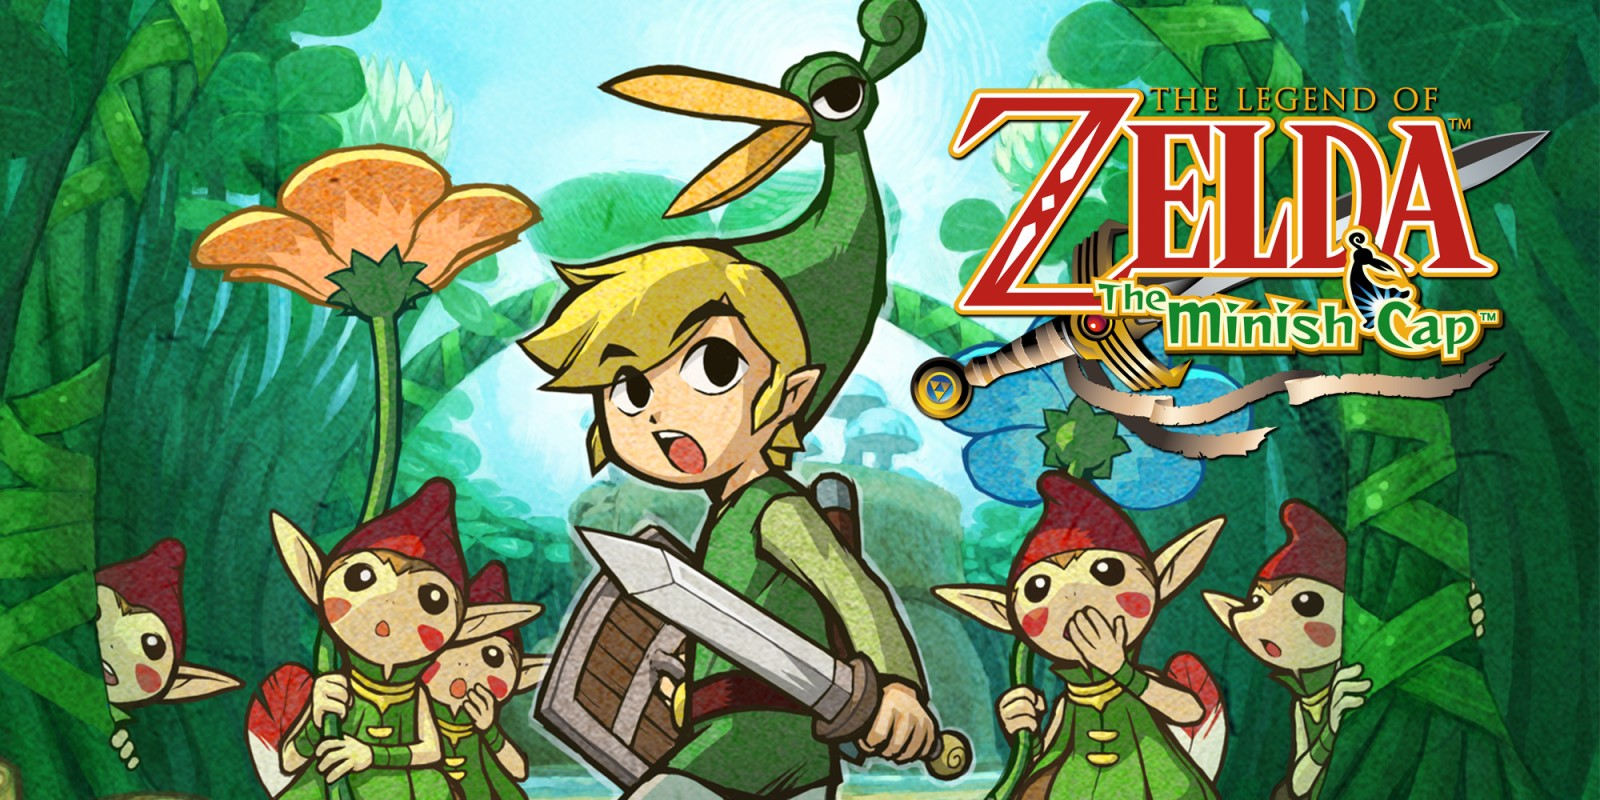
\includegraphics[width=0.6\textwidth]{Images/SI_GBA_TheLegendOfZeldaTheMinishCap_image1600w.jpg}
        \caption{The Legend Of Zelda Minish Cap}
        \label{fig:Zelda}
    \end{figure}

    Nótese también que esos videojuegos, salvo el último son videojuegos en 2 dimensiones que tienen una vista igual o similar a la presentada en Eldoria, es por ello que bebe mucho el TFG, de este tipo de fórmula que 
    a dia de hoy, juegos grandes siguen usando, sin ir más lejos, \textit{The legend of Zelda Tears of the Kingdom}, sigue la fórmula del primero juego, varias mazmorras, en las que el jugador se enfrenta a varios puzzles,
    antes de llegar al jefe final del juego, debe pasar por varias pruebas e incluso optar a conseguir un arma legendaria para hacerle frente.

    \subsection{Final fantasy}
    La segunda inspiración tomada es otro juego de los años 80, el cual se llama \textit{Final Fantasy}, este juego se trata de un juego en dos dimensiones RPG por turnos que nos presenta una historia,
    acerca de 4 muchachos que se embarcan en la búsqueda de unos cristales mágicos que les servirán para disipar el mal de su mundo, durante la aventura se enfrentan a enemigos formidables y el juego tiene
    una estética de fantasía medieval. A dia de hoy esta saga sigue en desarollo, actualmente han sacado 16 juegos principales y varios secundarios.
    Pero, al igual que en el caso de la saga Zelda, encontramos la misma estructura que se repite en mayor o menor medida a lo largo de sus videojuegos, y de nuevo, en esta saga en lo que nos inspiramos es el ambiente,
    el ambiente medieval de fantasía tirando más a fantasia en este caso. Si bien es cierto que algún videojuego de esta saga, toca temas bastante profundos, nosotros en nuestro desarrollo hemos obviado realizar una historia
    relativamente compleja, ya que nos llevaría mucho más tiempo de lo normal. Un ejemplo de ello sería el \textit{Final Fantasy VII}, el cual es considerado uno de los mejores videojuegos de la historia, trata varios temas
    dificiles y complejos, y sigue teniendo la fórmula clásica tan característica de esta saga.

    \begin{figure}[ht]
        \centering
        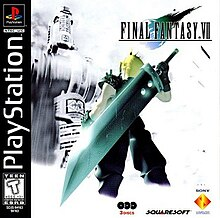
\includegraphics[width=0.6\textwidth]{Images/Final_Fantasy_VII_Box_Art.jpg}
        \caption{Final Fantasy VII}
        \label{fig:finalfantasy}
    \end{figure}

    \subsection{Blasphemous}
    La tercera inspiración ha sido un juego que se sale de los generos de RPG, se trata de un juego metroidvania, desarrollado en España, se trata de \textit{Blasphemous},
    un juego en dos dimensiones que nos pone en la piel del penitente, el cual entrará en un camino de penitencia y tendrá que realizar humillaciones para devolver el orden a su mundo, Cvstodia.
    Este juego presenta inspiración en mi proyecto ya que se trata de un juego con estética \textit{pixel art}, que es relativamente reciente. Este videojuego nos ha servido de inspiración ya que,
    al visualizar el documental acerca de como se ha desarrollado el juego, el cual hemos adjuntado en la bibliografía, podemos observar las complicaciones del mundo real, cuando queremos desarrollar un juego indie.
    Vemos como el tiempo siempre está ahí, como a veces, falta financiación, o como simplemente el equipo de desarrolladores se estresa mucho por las fechas limite.

    \begin{figure}[ht]
        \centering
        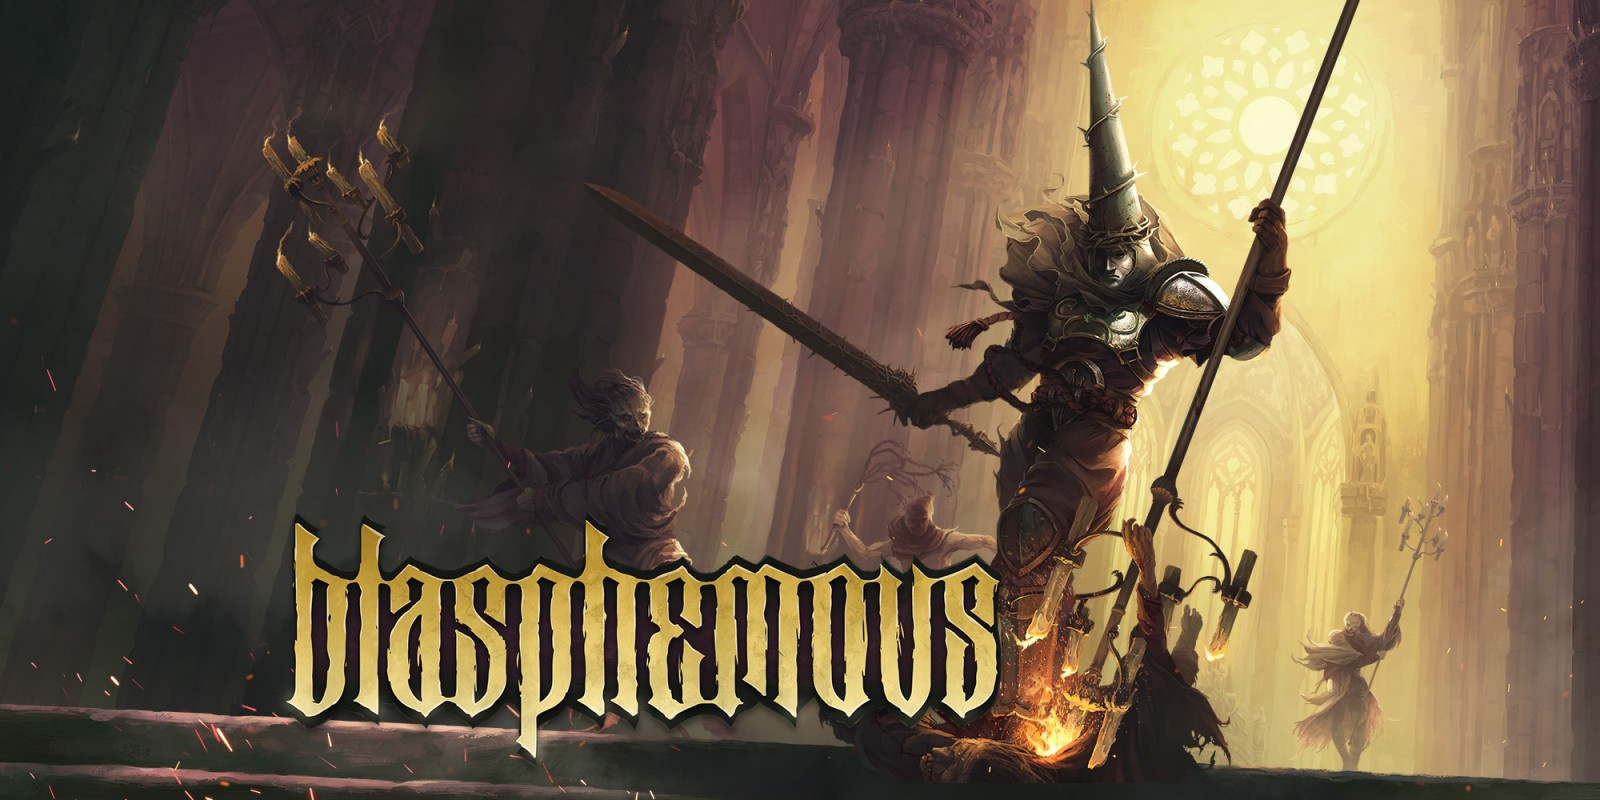
\includegraphics[width=0.6\textwidth]{Images/H2x1_NSwitchDS_Blasphemous_image1600w.jpg}
        \caption{Imagen de blasphemous}
        \label{fig:blasphemous}
    \end{figure}

    Es un documental que enseña, digamos, la cara oculta de desarrollar un videojuego, y esa cara oculta, son el estrés, la ansiedad, el no poder hacer quizás determinadas cosas por falta de tiempo, etc \dots
    Si bien es cierto que al final el producto que ha sacado este equipo de desarrolladores, ha sido una obra de una calidad muy alta, a mi me ha servido como mensaje de que se puede lograr lo que te propongas, con mucho esfuerzo,
    aparte de inspiración, ha sido una motivación que me ha llevado a realizar este TFG, además el videojuego al ser creado por un equipo Español, me ha animado mucho más.\\

    \begin{flushright}
        \textit{El equipo detrás del desarrollo de este videojuego fue The Game Kitchen}
    \end{flushright}
    \subsection{Arte del juego}
    El arte del juego sería una mezcla de todos los juegos ya mencionados excepto Blasphemous, ya que este último cuenta con sprites muy bien detallados y de mayor resolución.
    Se supone que el juego se desarrolla en una época medieval en la que existen magias, caballeros, dragones, ciclopes, etc \dots \\
    La mayoría de videojuegos de esta índole se desarrollan en épocas similares, remontandose en su mayoría al medievo europeo, o mundos mediavales con toques de fantasía que
    añaden juego a la hora de poder crear historias, personajes, escenarios, etc \dots \\
    Algunos ejemplos, aparte de los ya nombrados que siguen esta estética, podrían ser:

    \begin{itemize}
        \item Sea of stars
        \item Terraria
        \item Fire Emblem la saga completa
        \item V rising
    \end{itemize}

    \clearpage
    % ---------------------------------------

    \section{Anexo IV - Vocablos usados}
    Durante este documento se han hecho uso de varios vocablos de los que seguramente se desconozca el significado, tales como "FPS" por ejemplo, por ello vamos a recopilarlos aqui junto a su definicion.
    \begin{itemize}
        \item FPS Frames per second - Imágenes que dibuja el programa por segundo, un frame es toda la imagen que dibuja el programa entera, con el personaje, el mapa, los objetos, etc \dots
        \item RPG Role playing game - Acrónimo asociado a los juegos de Rol
        \item NPC Non Playable Character - Personaje no jugable, suelen ser personajes con los que podemos hablar o Interactuar
        \item Inputs - Se refiere a las entradas del usuario al programa
        \item Pixel art - Estética basada en dibujar con pixeles solamente sin ningun arco o elemento circular
        \item Retro - Se refiere a una estética antigua, por ejemplo la de los juegos de los años 80
        \item Sprites - Son un conjunto de imágenes que representan un objeto o personaje
        \item Aspect ratio - La relación de aspecto es la proporción entre el ancho y la altura de una imagen, pantalla o cuadro visual. Se expresa como una relación matemática, por ejemplo, 16:9 o 4:3, donde el primer número representa el ancho y el segundo número la altura.
        \item Farming - En videojuegos se refiere a la práctica de repetir ciertas acciones o actividades en el juego con el objetivo de obtener recursos, experiencia, ítems, dinero del juego, o cualquier otro tipo de recompensa. Esta actividad es común en muchos géneros de videojuegos, especialmente en juegos de rol (RPG), juegos de estrategia, y juegos multijugador en línea masivos (MMO)
    \end{itemize}
    \clearpage
    % ---------------------------------------

\end{appendices}

\end{document}